\section{Эксперименты}

В этой части работы мы будем эксперименталено изучать статистическую неопределлённость различных сетевых структур. Перед нами стоят две задачи: понять, как отклонение от нормального распределения влияет на статистическую неопределённость и изучить статистическую неопределённость структур, построенных на основе новой меры близости - вероятности совпадения знаков.

Таким образом, экспериментальная часть будем состоять из двух частей. В первой части в качестве меры близости мы применяем выборочную корреляцию Пирсона, во второй - вероятность совпадения знаков. Каждая из частей эксперимента включает в себя оценку статистической неопределённости каждой из структур  при различных значениях коэффициента $r$ смешанного распределения. 
Список изучаемых структур придставлен ниже:
\begin{itemize}
	\item Максимального остовного дерева (maximum spanning tree)
	\item Рыночного графа (market graph)
	\item Максимальной клики на основе рыночного графа (maximum clique)
	\item Максимального независимого множества на основе рыночного графа (maximum independent set)
\end{itemize}


Как и в [ссылка на нашу статью] мы будем оценить статистическую неопределённость, основываясь на $\mathcal{E}(\mathcal{S},n)$-мере по следующему алгоритму: 
\begin{enumerate}
	\item Построить эталонную структуру на основе имеющихся данных
	\item Сгенерировать выборку доходностей акций $x_{1 1}, ..., x_{1 N}, ..., x_{n 1}, ..., x_{n N}$
	\item Рассчитать матрицу весов на основе меры близости и сгенерированных наблюдений
	\item Построить выборочную сеть
	\item В выборочной сети построить выборочную сетевую структуру
	\item Рассчитать долю ошибок I($\frac{X_1}{M_1}$) и II рода($\frac{X_2}{M_2}$) , а также общую долю ошибок $X$
	\item Повторить 500 раз шаги 2-5 и рассчитать среднее общей доли ошибок $X$. Полученное значение и будет являться оценкой меры $\mathcal{E}(\mathcal{S},n)$.
\end{enumerate}

Генерация выборки доходностей акций из смешанного распределения происходит следющим образом. В функцию генерации \verb|mixed_t_normal| кроме параметров, необходимых для генераторов из многомерного нормального распределения и многомерного распределения Стьюдента, описанных [ГДЕ-то Выше Наверно], передаётся число наблюдений $n$ и параметр $r \in [0,1]$, которые отвечает за то, какая часть из $n$ наблюдений будет сгенерирована из многомерного распределения Стьюдента. Оставшая часть будет сгенерирована из многомерного нормального распределения. Например, если при $n=100$ и $r=0.3$ 30 наблюдений будет сгенерировано из многомерного распределения Стьюдента, а 70 -из многомерного нормального распределения. При $r=0$ - все наблюдения будут сгенерированы из многомерного нормального распределения, а при  $r=1$ - все наблюдения будут сгенерированы из многомерного распределения Стьюдента. 

В качестве генератора многомерного нормального распределения  была использована функция \verb|random.multivariate_normal()| библиотеки Numpy. Генератор 
многомерного распределения Стьюдента реализует описанные в [Где-то сверху] выражения с помощью функций \verb|random.multivariate_normal()| и  \verb|random.chisquarel()| [ссылка на доку] библиотеки Numpy.

Рассмотрим более детально алгоритмы построения сетевых структур, а также специфику вычисления их статистической неопределённости.


Для построения максимального остовного дерева была использована  функция \verb|algorithms.tree.mst.maximum_spanning_tree()| библиотеки NetworkX[ссылка на доку]. Она реализует алгоритм Краскала[ссылка на алгоритм] построение минимального остовного дерева, который итеративно строит остовное дерево, на каждом шаге присоединяя ребро наименьшего веса, добавление которого не вызовет появления цикла. Алгоритм может быть использован и для поиска максимального остовного дерева,  выбирая на каждом шаге ребро наибольшего веса.

Остовное дерево, полученное как из эталонной, так и из выборочной сети, содержит $N$ вершин и $M_1 = M_2 = N-1$ рёбер. Так вершины соединяет только одно ребро, если существует ребёро $(i,j)$, которое ошибочно включено в выборочную структуру( $x^{i j}_1=1$), то существует и ребро  $(k,s)$, котороя ошибочно не включено в структуру ( $x^{k s}_2=1$) и наоборот. Таким образом, ошибки I и II рода эквиваленты, а общая доля ошибок может быть найдена как
\begin{equation}
X = \frac{1}{2}\left(\frac{X_1}{M_1} + \frac{X_2}{M_2}\right) = \frac{X_1 + X_2}{2(N-1)} = \frac{X_1}{N-1}
\end{equation}



Построение рыночного графа не потребовало использования никаких специальных алгоритмов. Рыночный граф легко получить, отфильтровав список рёбер по весу.
Для рыночного графа значения $M_1$ и $M_2$ по-прежнему константные, и равные $\binom{N}{2} - M$ и $M$ соответнственно, где $M$ - количество рёбер в эталонном рыночном графе с некоторым выбранным значением порога $\theta$, а $\binom{N}{2}$ - число всех возможных рёбер в графе с $N$ вершинами. Общая доля ошибок $X$ для рыночного графа равна:

\begin{equation}
X = \frac{1}{2}\left(\frac{X_1}{M_1} + \frac{X_2}{M_2}\right) = \frac{1}{2}\left(\frac{X_1}{\binom{N}{2} - M} + \frac{X_2}{M}\right)
\end{equation}


Максимальная клика и максимальное независимое множество строятся на основе полученного рыночного графа. Так как таких структур в графе может быть несколько, для оценки неопределённости, мы будем искать максимальную клику с максимальным весом (maximum clique with maximal weight) и максимальное независимое множество с минимальным весом (maximum independent set with minimal weight).  

Для поиска максимальной клики с максимальным весом в графе была использована функция \verb|algorithms.clique.find_cliques()| библиотеки NetworkX[ссылка на доку], которая возвращает список всех клик графа, каждая из которых является кортежем из вершин графа, входящих в клику. Реализация поиска основана на алгоритме Брона — Кербоша(ССЫЛКА) для поиска всех клик в неориентированном графе.Полученный список сортируется по размеру клик(числу элементов в кортеже), а потом из клик максимального размера выбирается клика с наибольшим весом. Вес клики определяется суммой весом рёбер рыночного графа, которые соединяют вершины, входящие в клику.


Так как максимальное независимое множество графа совпадает с максимальном кликой в обратном графе, поиск максимального независимого множество реализован через поиск максимальной клики в дополнении рыночного графа. Дополнением графа $G$ является граф, в котором две вершины являются смежными, если они не смежны в исходном графе. Множество вершин у исходного графа и его дополнения совпадают, а объединённые множества рёбер обоих графов составляет множество рёбер полного графа на этом множестве вершин. Дополнение графа также называют обратным графом (ССЫЛКА). Таким образом, чтобы найти максимальное независимое множество графа, можно применить описанный выше подход для поиска максимальной клики в дополнении рыночного графа, только вместо максимальной клики с наибольшим весом будем выбирать клику с наименьшим весом.

В отличие от максимального оставного дерева и рыночного графа значения $M_1$ уже не является константой, так как размер выборочной максимальной клики может изменяться. Теперь $M_1 = \binom{C_s}{2}$, а $M_2 = \binom{C_r}{2}$, где $C_s$ - число веришн в выборочной максимальной клике, а $C_r$ - число веришн в эталонной. Значение $C_r$ - константа.

\begin{equation}
X = \frac{1}{2}\left(\frac{X_1}{M_1} + \frac{X_2}{M_2}\right) = \frac{1}{2}\left(\frac{X_1}{\binom{C_s}{2}} + \frac{X_2}{\frac{X_2}{\binom{C_r}{2}}}\right)
\end{equation}


Алогоритм вычисления ошибок I и II рода ($X_1$ и $X_2$) одинаковый для каждой из структур. Он состоит в использовании функции  \verb|algorithms.operators.difference()| библиотеки NetworkX[ссылка на доку]. Эта функция принимает на вход два графа и возвращает граф с тем же множеством вершин  и множеством рёбер, которые содержатся в первом графе, но не содержатся во втором. У полученного графа мы считаем количество рёбер. Таким образом, передавая в функцию выборочную структуру первым аргументов, а эталонную вторым, мы получаем ошибку I рода. Передавая структуры в обратном порядке, получаем ошибку II рода


\subsection{Анализ эталонной сети}

Данными для эскперимента являются 470 наблюдений за $N=100$ акциями NASDAQ в период 2018-2019 годов. На основании этих данных, построим матрицу выборочной корреляции Пирсона $||\rho_{i j}||$ и матрицу вероятностей совпадения знаков, которые будут являться матрицами весов для эталонных сетей. К ним мы будем применять различные процедуры фильтрации и получать эталонные сетевые структуры, с помощью которых мы будем оценивать статистическую неопределённость.

Данные были загружены с помощью библиотеки Yahoo! Finance market data downloader [ссылка на доки]. Набор тикеров был получен путём веб-скрейпинга сайта http://eoddata.com.

Рассмотрим некоторые статистики эталонных сетевых структур с\textbf{ корреляцией Пирсона} в качестве меры близости. В таблице \ref{table:mg_size} отображена зависимость числа рёбер от выбранного порога $\theta$ в эталонном рыночном графе.

\begin{table}[h!]
\centering
\begin{tabular}{ |c|c|c|c|c|c|c|c|c|c| } 
 \hline
 $\theta$ & -1 & 0 & 0.1 & 0.2 & 0.3 & 0.4 & 0.5 & 0.6 & 0.7 \\ 
 \hline
 |E|	  & 4950 & 4584 & 3593 & 2282 & 1108 & 428 & 150 & 51 & 16\\ 
 \hline
\end{tabular}
\caption{Зависимость числа рёбер в рыночном графе от $\theta$}
\label{table:mg_size}
\end{table}


В таблице \ref{table:mis_clique_size} приведены размеры максимальной клики и максимального независимого множества в эталонном рыночном графе в зависимости от выбранного порога $\theta$.

\begin{table}[h!]
\centering
\begin{tabular}{ |c|c|c|c|c|c|c|c|c| } 
 \hline
 $\theta$ & 0 & 0.1 & 0.2 & 0.3 & 0.4 & 0.5 & 0.6 & 0.7 \\ 
 \hline
 N clique & 81 & 64 & 43 & 24 & 15 & 10 & 5 & 3\\ 
 \hline
 N mis    & 5  & 14 & 29 & 41 & 60 & 76 & 84 & 92\\ 
 \hline
\end{tabular}
\caption{Зависимость размеров структур от $\theta$}
\label{table:mis_clique_size}
\end{table}

На рисунке \ref{fig:ref_graph_p} изображён эталонный рыночный граф с порогом $\theta=0.5$, а также максимальная клики и максимальное независимое множество этого графа. Вершины, входящие в клику изображены синим цветом, входящие в независимое множество - красным.

\begin{figure}[H]
\centering
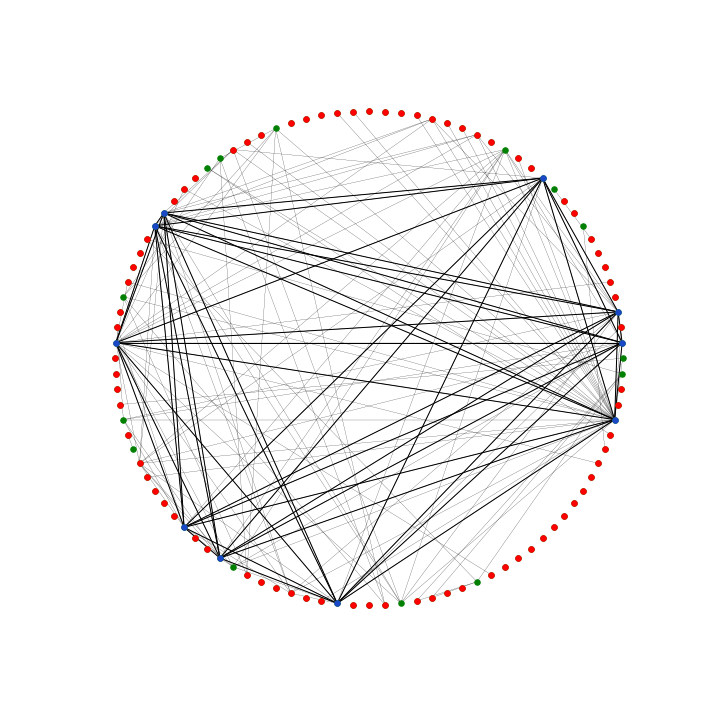
\includegraphics[scale=0.4]{ref_graph_p}
\caption{Эталонный рыночный граф с порогом $\theta=0.5$}
\label{fig:ref_graph_p}
\end{figure}



Теперь рассмотрим те же статистики эталонных сетевых структур, но с\textbf{ вероятностями совпадения знаков} в качестве меры близости. Порог $\theta$ преобразован в $\theta_\gamma$ согласно (\ref{eq:threshold}). 

В таблицах \ref{table:mg_size_sign} и \ref{table:mis_clique_size_sign} отображены зависимость числа рёбер от выбранного порога и  размеры максимальной клики и максимального независимого множества.

\begin{table}[h!]
\centering
\begin{tabular}{ |c|c|c|c|c|c|c|c|c|c|c|c| } 
 \hline
 $\theta$ & -1 & 0 & 0.1 & 0.2 & 0.3 & 0.4 & 0.5 & 0.6 & 0.7 & 0.8 & 0.9 \\ 
 \hline
  $\theta_\gamma$ & 0 & 0.5 & 0.53 & 0.56 & 0.6 & 0.63 & 0.67 & 0.7 & 0.75 & 0.8 & 0.86 \\ 
 \hline
 |E|	  & 4950 & 3906 & 3299 & 2341 & 1299 & 554 & 226 & 83 & 26 & 10 & 2 \\ 
 \hline
\end{tabular}
\caption{Зависимость числа рёбер в рыночном графе от $\theta$ и $\theta_\gamma$}
\label{table:mg_size_sign}
\end{table}


\begin{table}[h!]
\centering
\begin{tabular}{ |c|c|c|c|c|c|c|c|c|c|c| } 
 \hline
 $\theta$ & 0 & 0.1 & 0.2 & 0.3 & 0.4 & 0.5 & 0.6 & 0.7 & 0.8 & 0.9 \\ 
 \hline
  $\theta_\gamma$ & 0.5 & 0.53 & 0.56 & 0.6 & 0.63 & 0.67 & 0.7 & 0.75 & 0.8 & 0.86 \\ 
 \hline
 N clique & 73 & 55 & 37 & 25 & 16 & 10 & 5 & 4 & 3 & 2\\ 
 \hline
 N mis & 14  & 18 & 29 & 38 & 52 & 68 & 80 & 88 & 95 & 98\\ 
 \hline
\end{tabular}
\caption{Зависимость размеров структур от $\theta$ и $\theta_\gamma$}
\label{table:mis_clique_size_sign}
\end{table}



\subsection{Измерение неопределённости сетевых структур}

Для каждой из структур будем применять две меры неопределённости: корреляция Пирсона и вероятность совпадения знаков.

Для корреляции Пирсона основным экспериментом будет измерение общей доли  ошибки в зависимости от числа наблюдений $n$ для различых параметром $r$. Таким образом, мы сможем изучить, как влияет на статистическую неопределённость отклонения от нормального распределения. Мы увидим, что чем ближе значения параметра $r$ к единице, то есть чем больше отклонение, тем больше общая доля ошибок для каждой из структур.

Для вероятности совпадения знаков мы рассмотрим зависимость  общей доли ошибки от параметра $r$ для различных значений параметра $r$ для различных значений числа наблюдений $n$. Так мы изучим влияние отклонения от нормального распределения на статистическую неопределённость структуры, построенной на вероятности совпадения знаков. Мы увидим, что подобного отклонения практически нет для любой из выбранных структур. Кроме того, мы сможем исследовать величину общей доли ошибки в зависимости от выбранной меры близости для выбранного значений $n$.

Доли ошибок для корреляции знаков мы сравним с ошибками для корреляции Пирсона при $r=1$ и $r=0$ как для случаев с наибольшей и наименьшей ошибками соответственно. Мы будем сравнивать с единственным значением ошибки для знаков, так как при изменении $r$ значение общей доли ошиюки будет оставаться практически неизменной. Для максимальной клики и максимального независимого множества помимо общей доли ошибки, будут также представлены доли ошибок I и II рода.

\subsubsection{Максимальное остовное дерево}

На рисунке \ref{fig:exp/mst/10k} представлен график зависимости общей доли ошибки от числа наблюдений для различных $r$. При $r=0$, то есть при генерации только из нормального распределения, порог $\mathcal{E}_0=0.1$ достигается примерно при $n=4000$ наблюдений, далее ошибка продолжает медленно убывать. В работе (ссылка) порог достигался при более чем 10000 набледедий.

\begin{figure}[H]
\centering
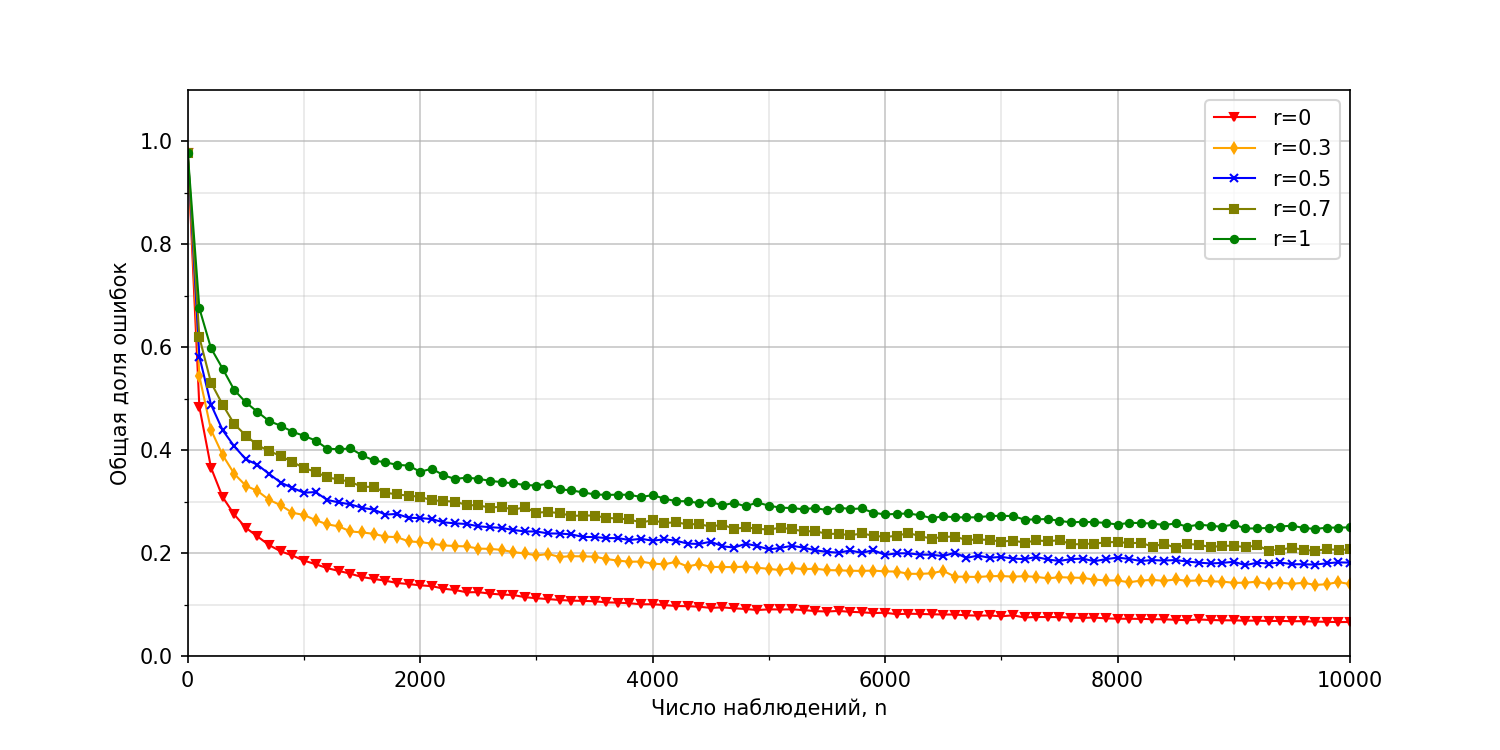
\includegraphics[scale=0.5]{mst/mst10k}
\caption{Зависимость общей доли ошибок от $n$, MST}
\label{fig:exp/mst/10k}
\end{figure}

На рисунке \ref{fig:exp/mst/pearson_ratio} представлен график зависимости общей доли ошибки от параметра $r$ при различных $n$. Уже при $r>0.1$ числа наблюдений $n=10000$ не хватает, чтобы достичь порога $\mathcal{E}_0=0.1$. 

\begin{figure}[H]
\centering
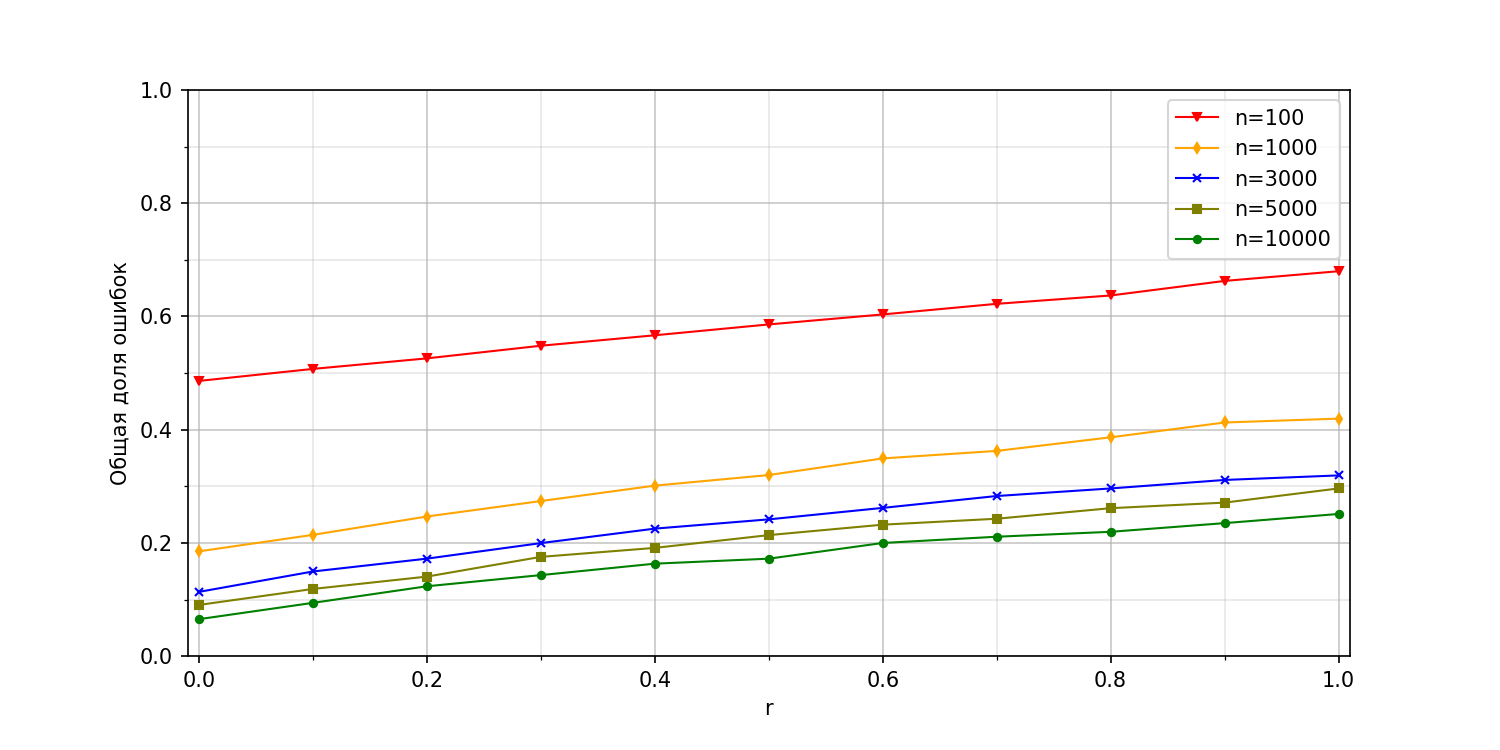
\includegraphics[scale=0.5]{mst/mst_pearson_ratio}
\caption{Зависимость общей доли ошибок от $r$, MST}
\label{fig:exp/mst/pearson_ratio}
\end{figure}

Теперь рассмотрим вероятность совпадения знаков в качестве меры близости. На рисунке \ref{fig:exp/mst/mst_signs_ration} представлен график зависимости общей доли ошибки от параметра $r$ при различных $n$. Видно, что изменения в распределении практически никак не влияют на значение ошибки. Однако  достичь порога $\mathcal{E}_0=0.1$ не получается даже при  $n=10000$. Судя по графику, значение общей доли ошибок стремится к 0.5 при увеличении числа наблюдений $n$. Подобная зависимость общей доли ошибки от параметра $r$ будет наблюдаться и для остальных структур, из чего мы сможем сделать вывод, что вероятность совпадения знаков устойчива к отклонениям наблюдений от нормального распределения подобного рода.

\begin{figure}[H]
\centering
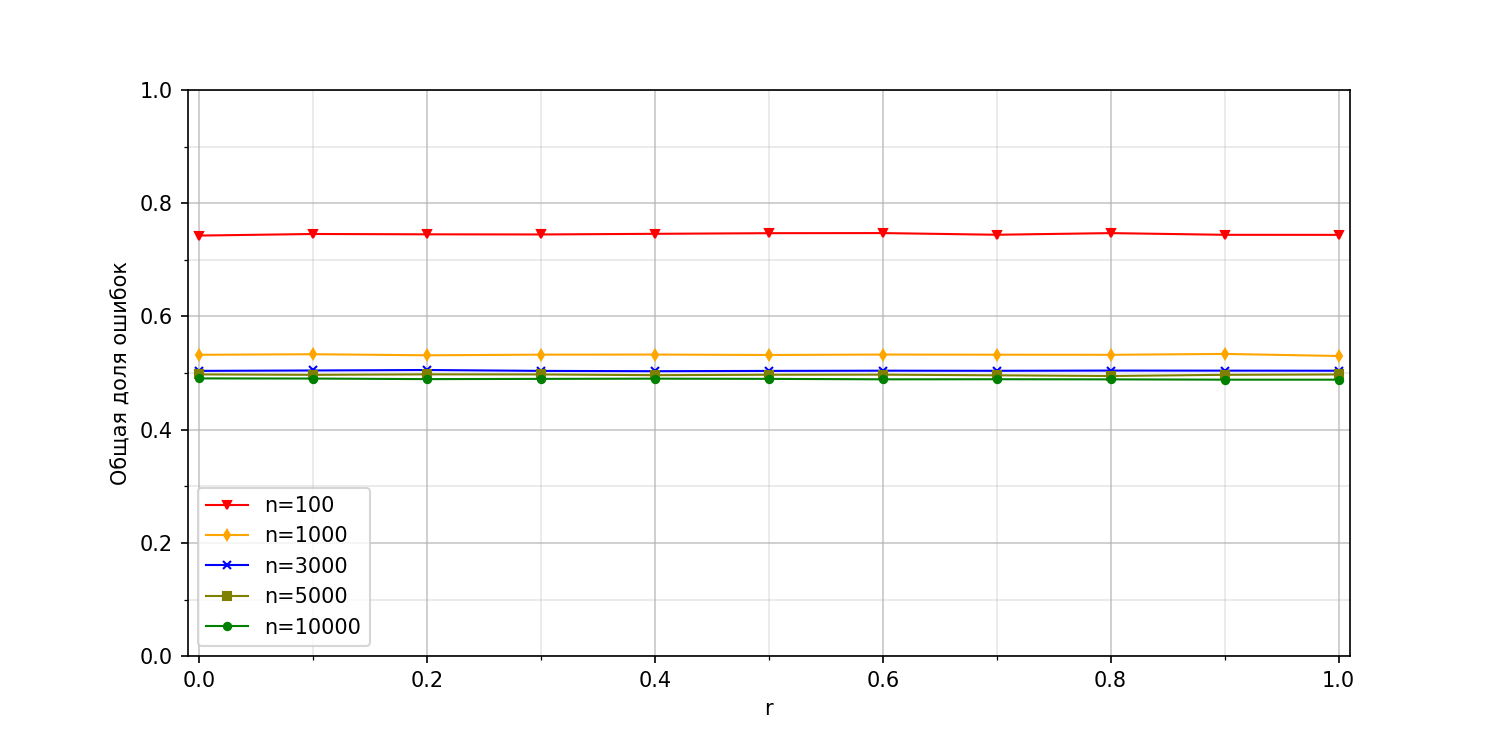
\includegraphics[scale=0.5]{mst/mst_signs_ration}
\caption{Зависимость общей доли ошибок от $r$ для знаков, MST}
\label{fig:exp/mst/mst_signs_ration}
\end{figure}

На слудеющем рисунке \ref{fig:exp/mst/pearson_signs} представлены графики сравнения неопределённости при использовании коррелиции Пирсона и вероятности выпадения знаков. Слева изображён график зависимости общей доли ошибки от параметра $r$ при различных $n$ для корреляции Пирсона и корреляции вероятности совпадения знаков. Справа - график, показывающий значения ошибки для корреляции Пирсона при $r=0$ и $r=1$ и для вероятности совпадения знаков, общая доля ошибок для которой сохраняется при изменении $r$. Видно, что даже при $r=1$, структура на основе корреляции Пирсона более стабильна.

\begin{figure}[H]
     \centering
     \begin{subfigure}[b]{0.49\textwidth}
         \centering
         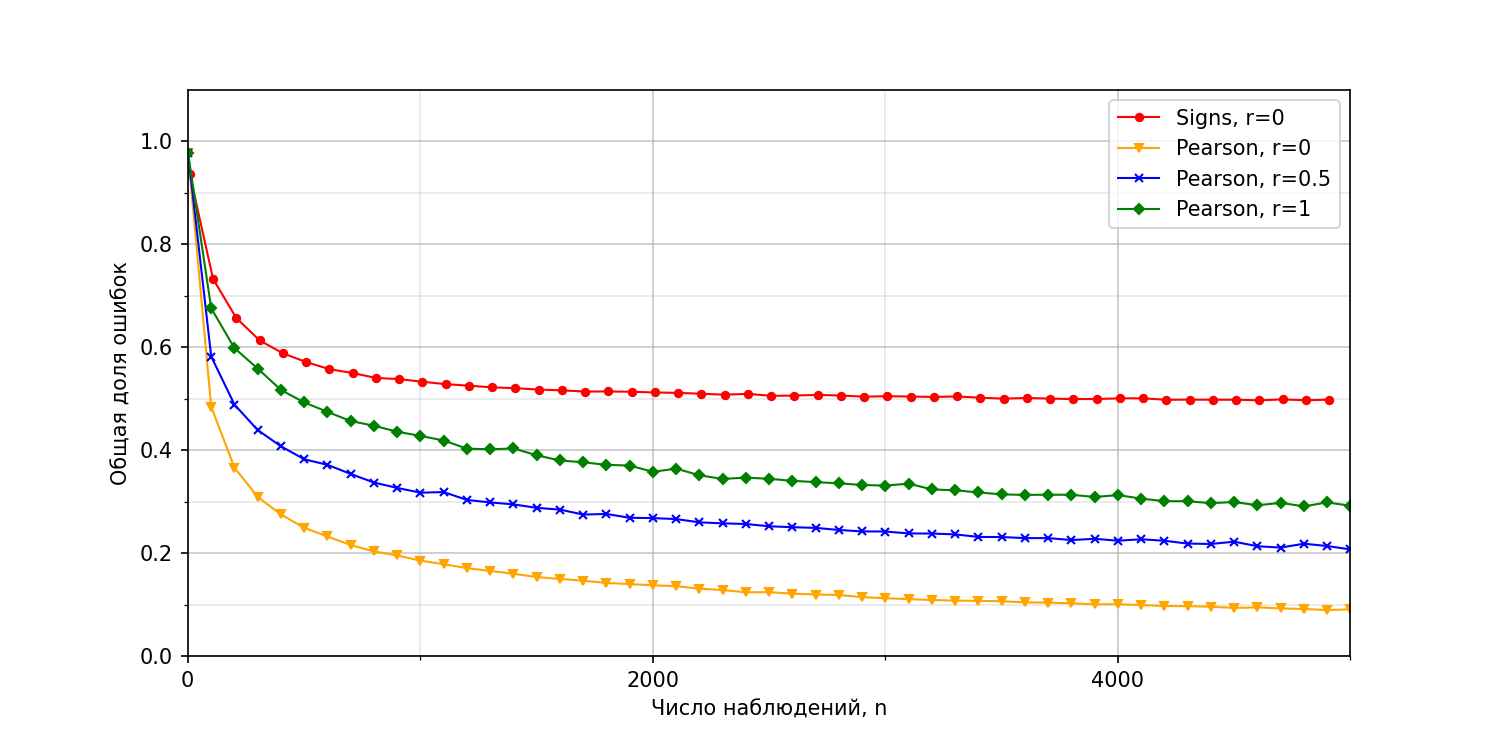
\includegraphics[width=\textwidth]{mst/mst10k_s_p}
     \end{subfigure}
     \hfill
     \begin{subfigure}[b]{0.49\textwidth}
         \centering
         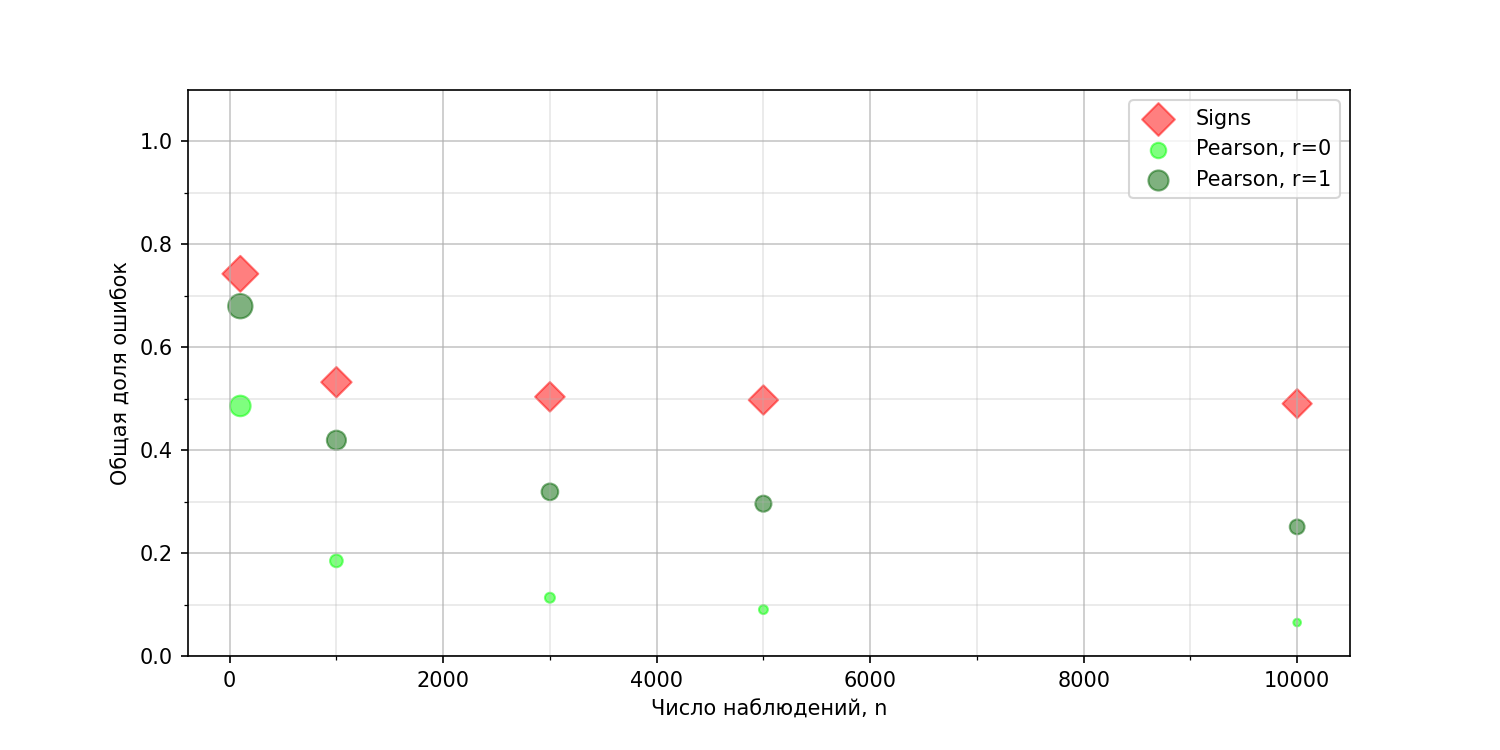
\includegraphics[width=\textwidth]{mst/person_signs}
     \end{subfigure}
     

        \caption{Зависимость общей доли ошибок от $n$, MST}
        \label{fig:exp/mst/pearson_signs}
\end{figure}  


\subsubsection{Рыночный граф}
В отличие от максимального остовного дерева рыночный граф имеет дополнительный параметр: порог $\theta$. Мы рассмотрим несколько значений порга $\theta$: $\theta \in [0.1, 0.3, 0.5, 0.7]$. Каждый график будет соответствовать своему значению $\theta$.

На рисунке \ref{fig:exp/mg/5k} представлен график зависимости общей доли ошибки от числа наблюдений для различных $r$ при различных значениях порога $\theta$. В отличие от максимального остовного дерева, уровень $\mathcal{E}_0=0.1$ достигается при гораздо меньшем числе наблюдений. При пороге выше $\theta=0.5$ уровень $\mathcal{E}_0=0.1$ достигается для любого значения $r$.


\begin{figure}[H]
     \centering
     \begin{subfigure}[b]{0.49\textwidth}
         \centering
         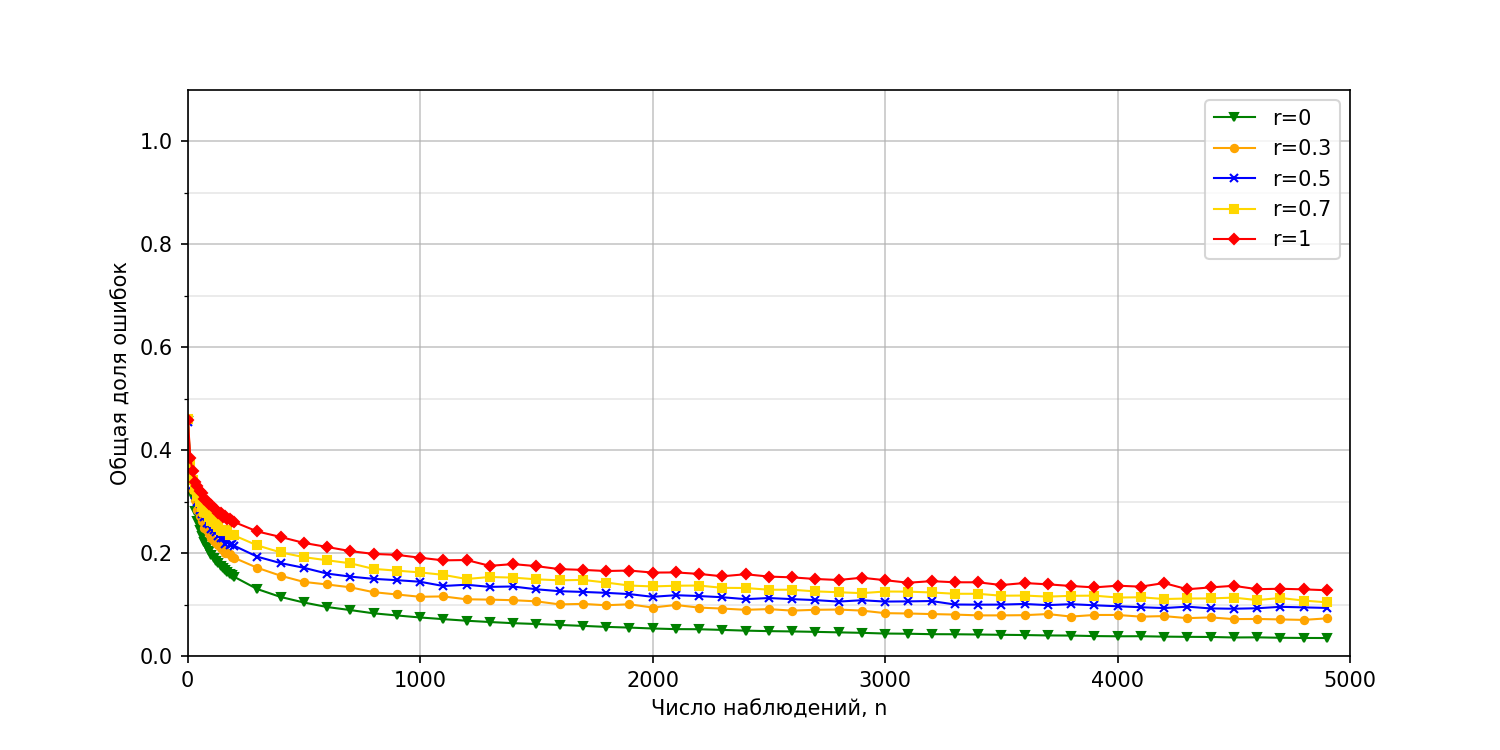
\includegraphics[width=\textwidth]{mg/pearson_5k_t=0-1}
         \caption{$\theta=0.1$}
     \end{subfigure}
     \hfill
     \begin{subfigure}[b]{0.49\textwidth}
         \centering
         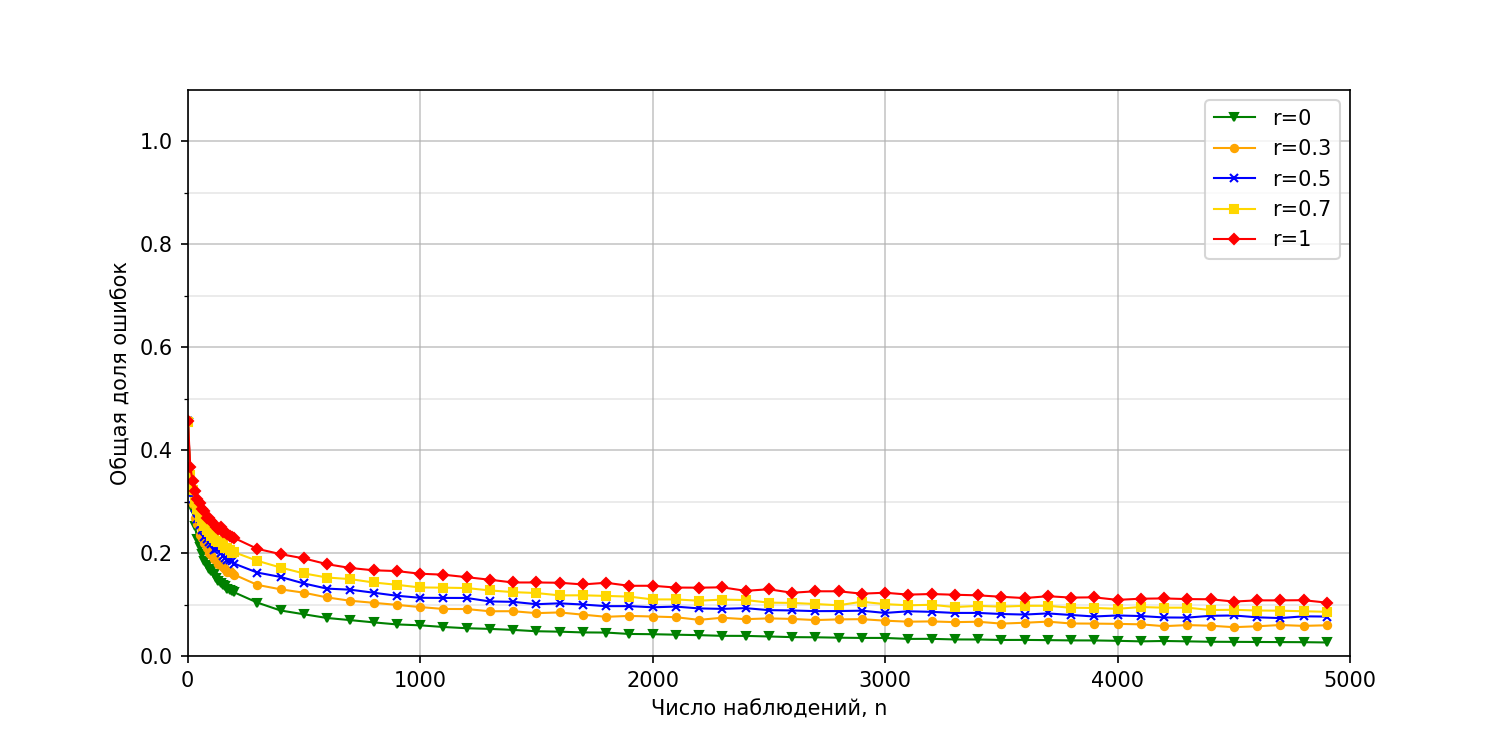
\includegraphics[width=\textwidth]{mg/pearson_5k_t=0-3}
         \caption{$\theta=0.3$}
     \end{subfigure}
     \vfill
     \begin{subfigure}[b]{0.49\textwidth}
         \centering
         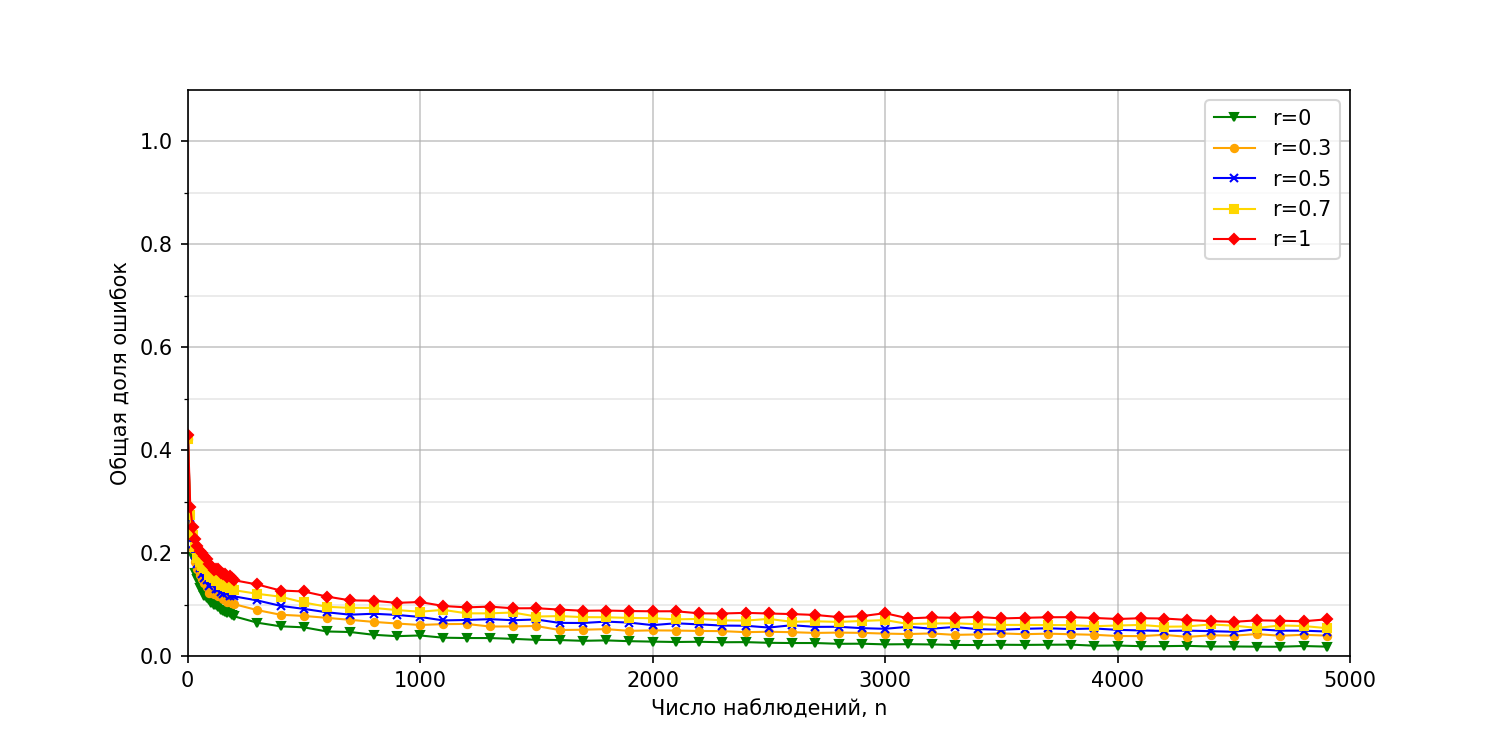
\includegraphics[width=\textwidth]{mg/pearson_5k_t=0-5}
         \caption{$\theta=0.5$}
     \end{subfigure}
     \hfill
     \begin{subfigure}[b]{0.49\textwidth}
         \centering
         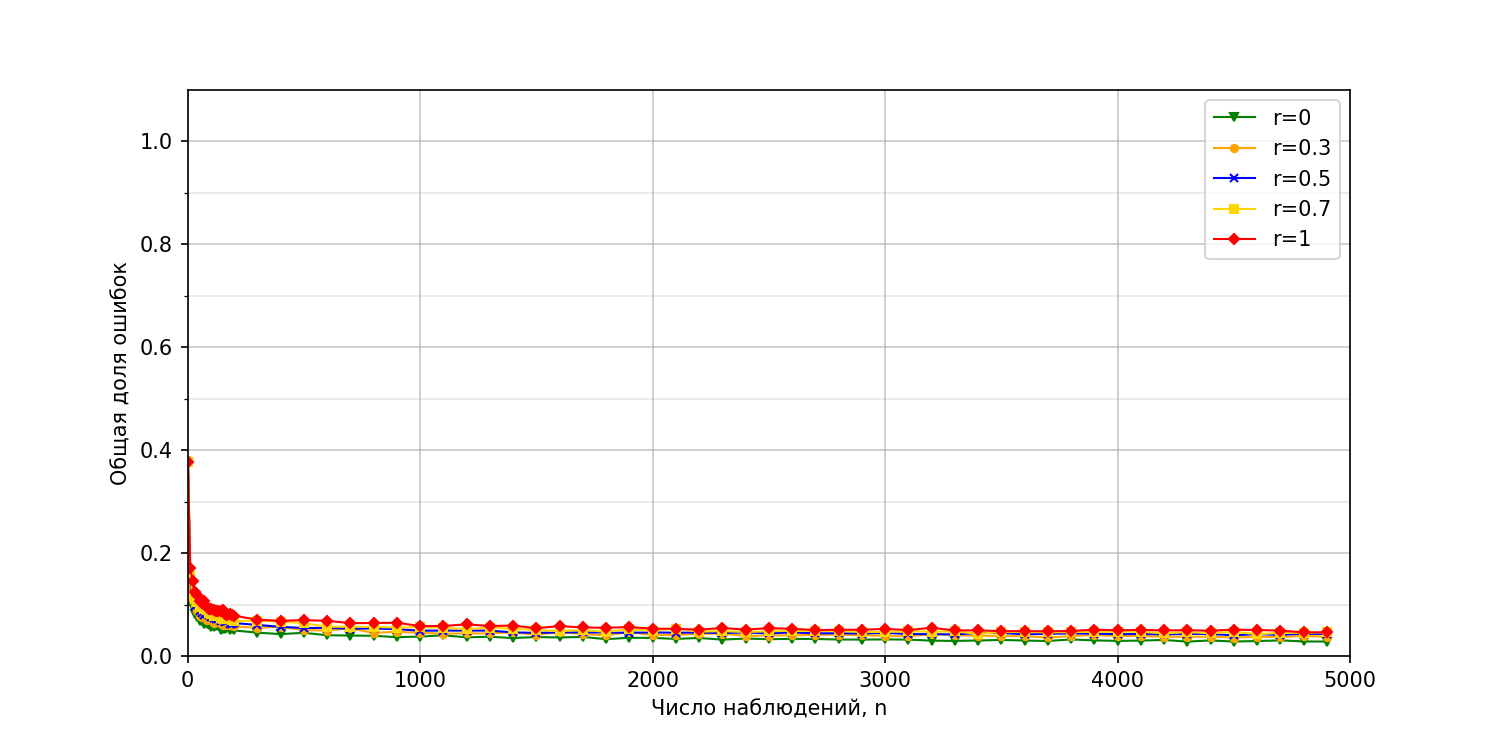
\includegraphics[width=\textwidth]{mg/pearson_5k_t=0-7}
         \caption{$\theta=0.7$}
     \end{subfigure}
     

        \caption{Зависимость общей доли ошибок от $n$, MG}
        \label{fig:exp/mg/5k}
\end{figure}  


Для меры близости на основе вероятности совпадения знаков на рисунке \ref{fig:exp/mg/signs_ration} представлен график зависимости общей доли ошибки от параметра $r$ при различных $n$. Как и для минимального остовного дерева, изменения в распределении также практически никак не влияют на значение ошибок. Достичь порога $\mathcal{E}_0=0.1$  всё также не удаётся, хотя общая доля ошибка меньше: около $\mathcal{E}=0.2$ для всех рассмотренных значений порога $\theta$. Согласно условию (\ref{eq:threshold}) при работе со знаками, мы преобразуем порог $\theta$ в $\theta_\gamma$. Значения $\theta_\gamma$ также представлено.


\begin{figure}[H]
     \centering
     \begin{subfigure}[b]{0.49\textwidth}
         \centering
         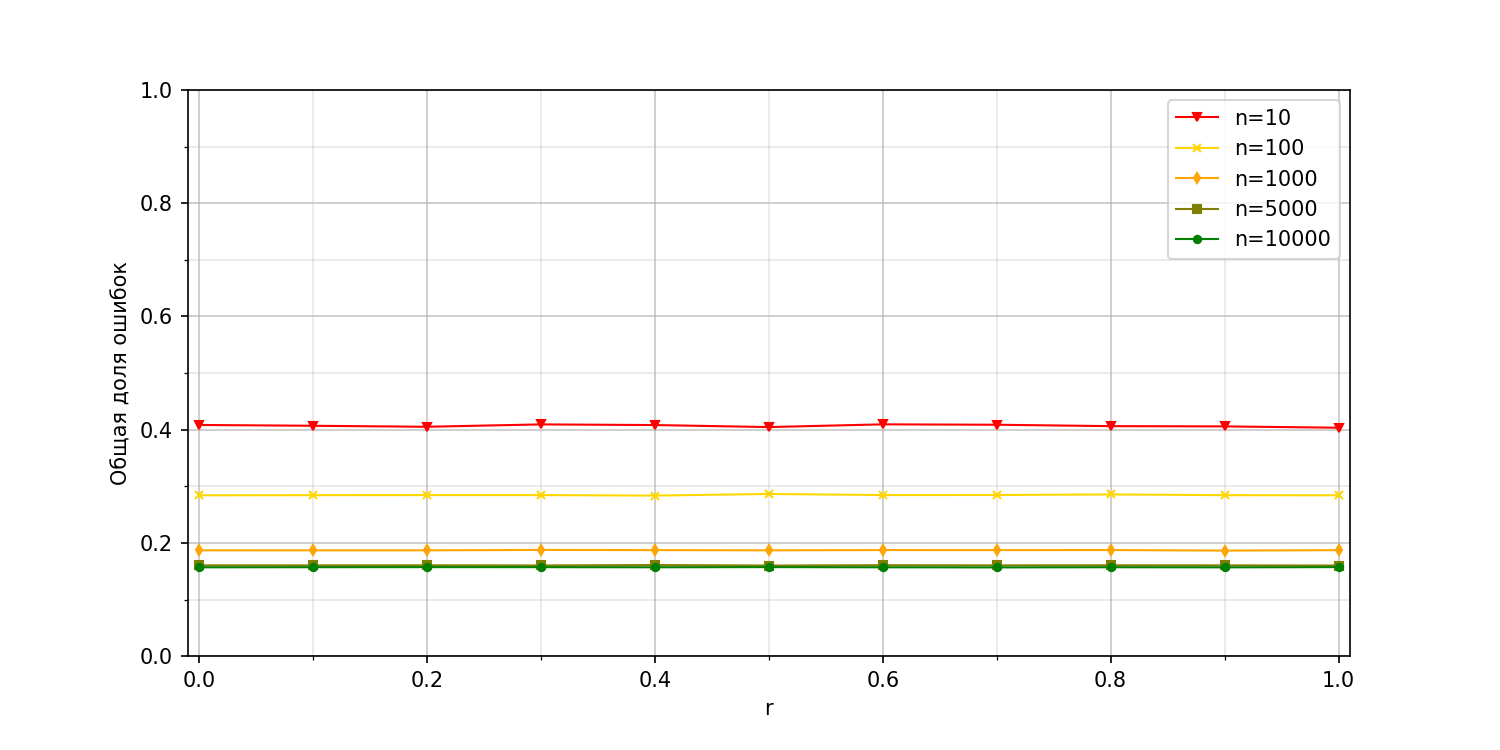
\includegraphics[width=\textwidth]{mg/signs_ratio_t=0-1}
         \caption{$\theta=0.1, \theta_\gamma=0.53$}
     \end{subfigure}
     \hfill
     \begin{subfigure}[b]{0.49\textwidth}
         \centering
         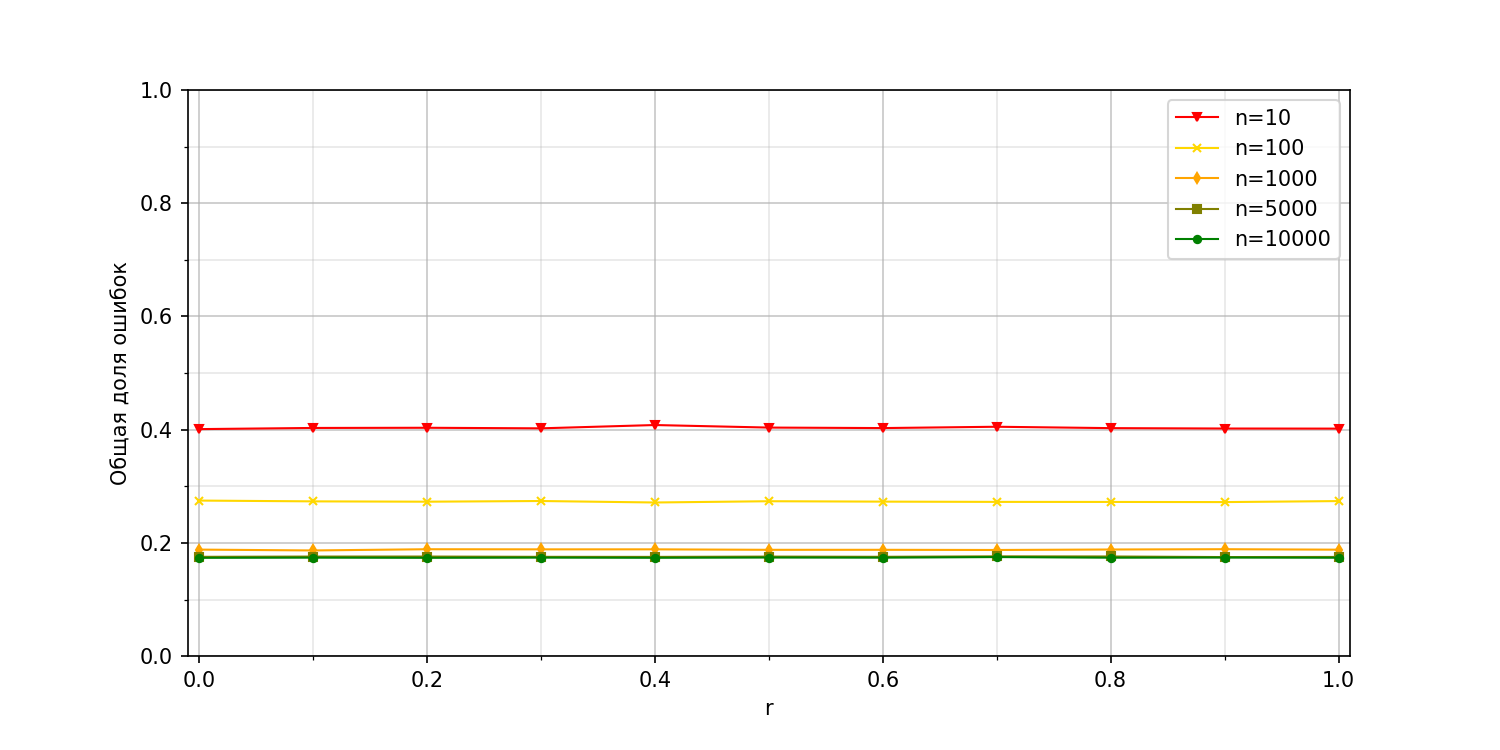
\includegraphics[width=\textwidth]{mg/signs_ratio_t=0-3}
         \caption{$\theta=0.3, \theta_\gamma=0.6$}
     \end{subfigure}
     \vfill
     \begin{subfigure}[b]{0.49\textwidth}
         \centering
         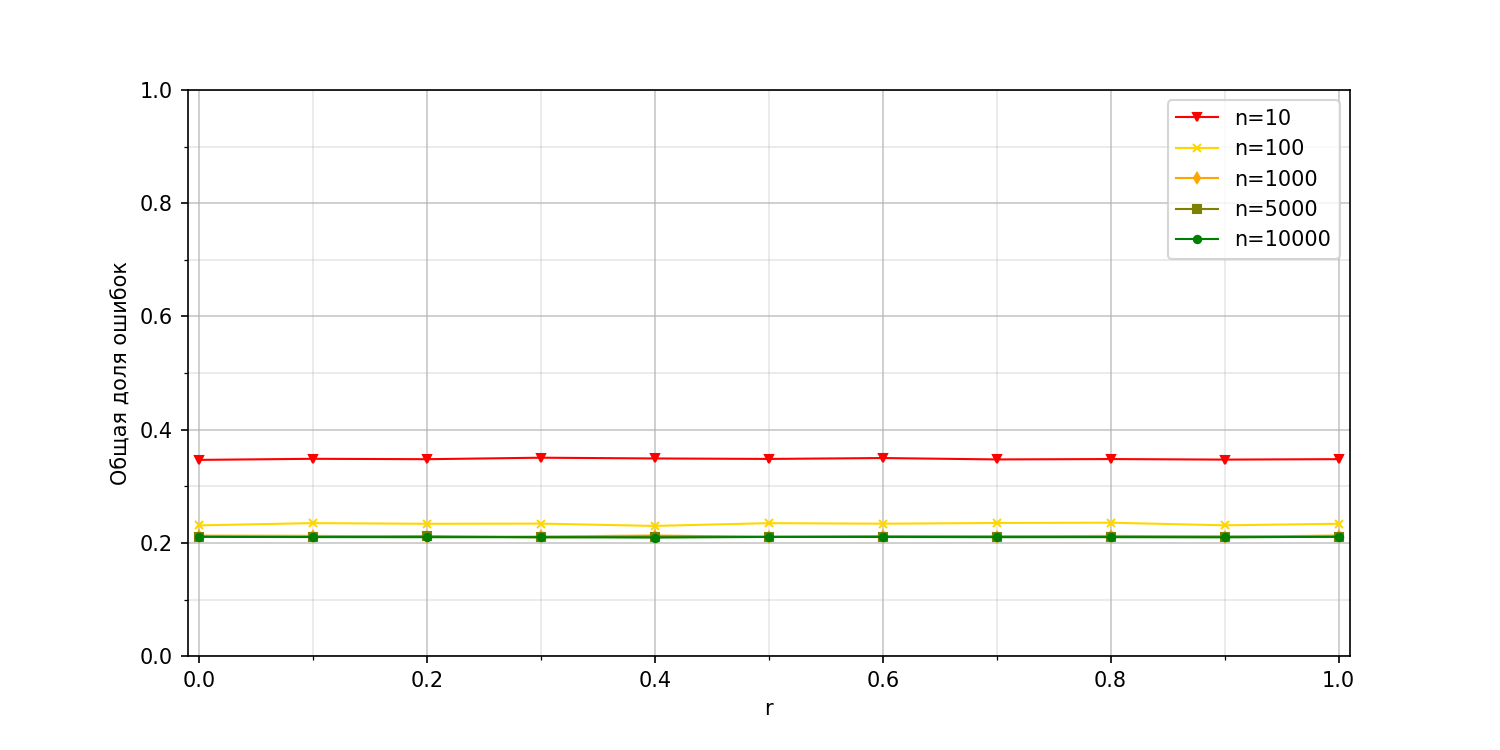
\includegraphics[width=\textwidth]{mg/signs_ratio_t=0-5}
         \caption{$\theta=0.5, \theta_\gamma=0.67$}
     \end{subfigure}
     \hfill
     \begin{subfigure}[b]{0.49\textwidth}
         \centering
         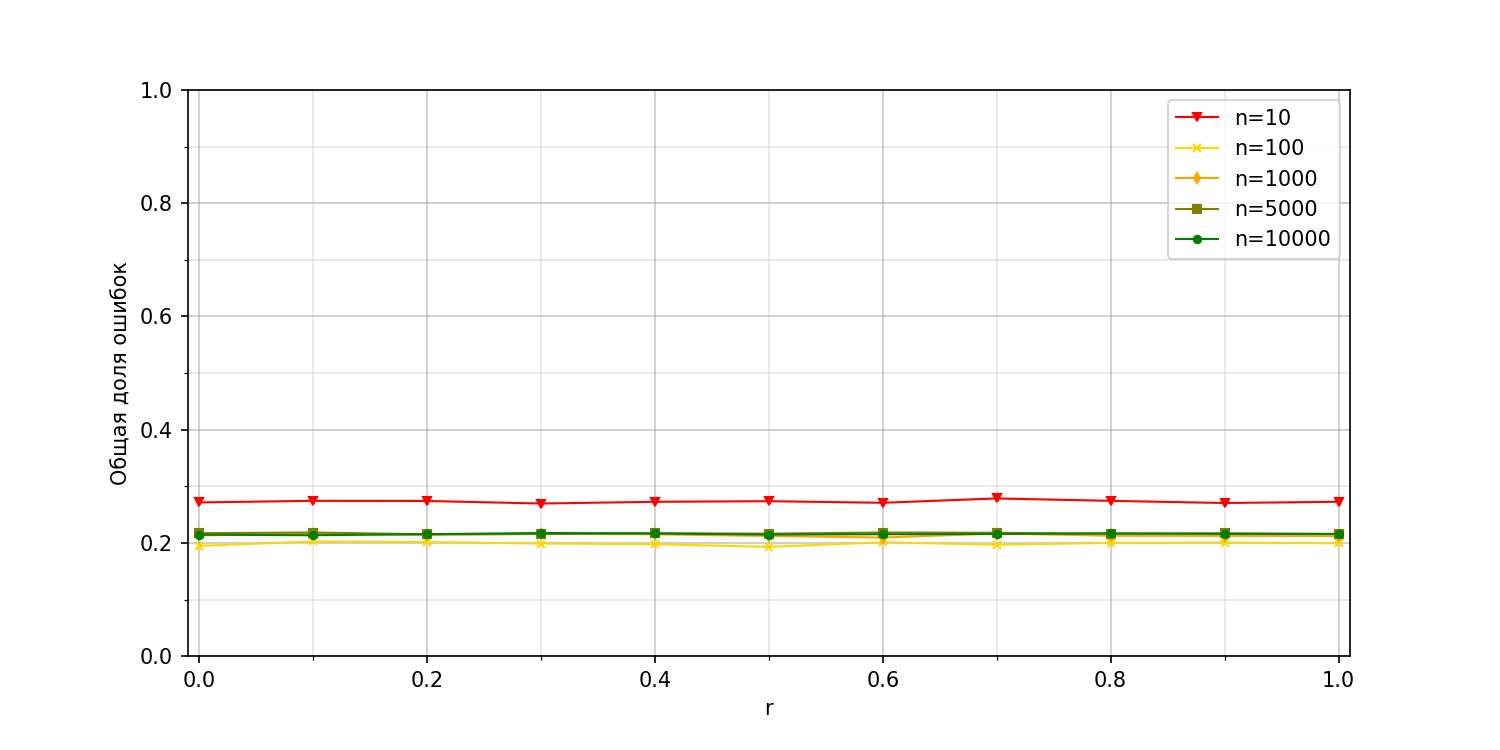
\includegraphics[width=\textwidth]{mg/signs_ratio_t=0-7}
         \caption{$\theta=0.7,\theta_\gamma=0.75s$}
     \end{subfigure}
     

        \caption{Зависимость общей доли ошибок от $r$ для знаков, MG}
        \label{fig:exp/mg/signs_ration}
\end{figure}  


На слудеющем рисунке \ref{fig:exp/mg/pearson_signs} представлены график сравнения ошибок при использовании корреляции Пирсона и корреляции вероятности совпадения знаков. Заметим, что при маленьких значениях $\theta$ ошибки для корреляции Пирсона при $r=1$ и корреляции знаков практически идентичны при разных $n$, однако при увеличии порого $\theta$ значения ошибки для корреляции Пирсона становится меньше. Это может быть вызвано преобразованием порога, либо тем, что знаки показывают себя лучше при использовании с маленьким $\theta$, то есть при большом количстве рёбер в сети.

\begin{figure}[H]
     \centering
     \begin{subfigure}[b]{0.49\textwidth}
         \centering
         \includegraphics[width=\textwidth]{mg/person_signs_t=0-1}
         \caption{$\theta=0.1, \theta_\gamma=0.53$}
     \end{subfigure}
     \hfill
     \begin{subfigure}[b]{0.49\textwidth}
         \centering
         \includegraphics[width=\textwidth]{mg/person_signs_t=0-3}
         \caption{$\theta=0.3, \theta_\gamma=0.6$}
     \end{subfigure}
     \vfill
     \begin{subfigure}[b]{0.49\textwidth}
         \centering
         \includegraphics[width=\textwidth]{mg/person_signs_t=0-5}
         \caption{$\theta=0.5, \theta_\gamma=0.67$}
     \end{subfigure}
     \hfill
     \begin{subfigure}[b]{0.49\textwidth}
         \centering
         \includegraphics[width=\textwidth]{mg/person_signs_t=0-7}
         \caption{$\theta=0.7,\theta_\gamma=0.75$}
     \end{subfigure}
     

        \caption{Сравнение ошибки для обеих мер, MG}
        \label{fig:exp/mg/pearson_signs}
\end{figure}  


\subsubsection{Максимальная клика}
Максимальная клика и максимальное назависимое множество строятся на основе рыночного графа.  Порог $\theta$ для максимальной клики будем брать из множества $\theta \in [0.1, 0.3, 0.5, 0.7]$.

На рисунке \ref{fig:exp/mc/total_1k} изображены графики зависимости общей доли ошибок от количества наблюдений $n$ для различных значений порога и, соответственно, для различных размеров клики.  Значение  общей доли ошибок остаётся достаточно большим, в сравнении со значениями ошибки в рыночном графе. Оно варьируется он $\mathcal{E}=0.2$ до  $\mathcal{E}=0.4$ в зависимости от значения $r$. При большом и маленьком порогах $\theta=0.7$ и $\theta=0.1$ значения ошибок меньше, чем при средних $\theta=0.3$ и $\theta=0.5$. При $\theta=0.7$ и $\theta=0.1$ достигается значение порога $\mathcal{E}_0=0.1$


\begin{figure}[H]
     \centering
     \begin{subfigure}[b]{0.49\textwidth}
         \centering
         \includegraphics[width=\textwidth]{mc/total/pearson_total_1k_t=0-1}
         \caption{$\theta=0.1, N=64$}
     \end{subfigure}
     \hfill
     \begin{subfigure}[b]{0.49\textwidth}
         \centering
         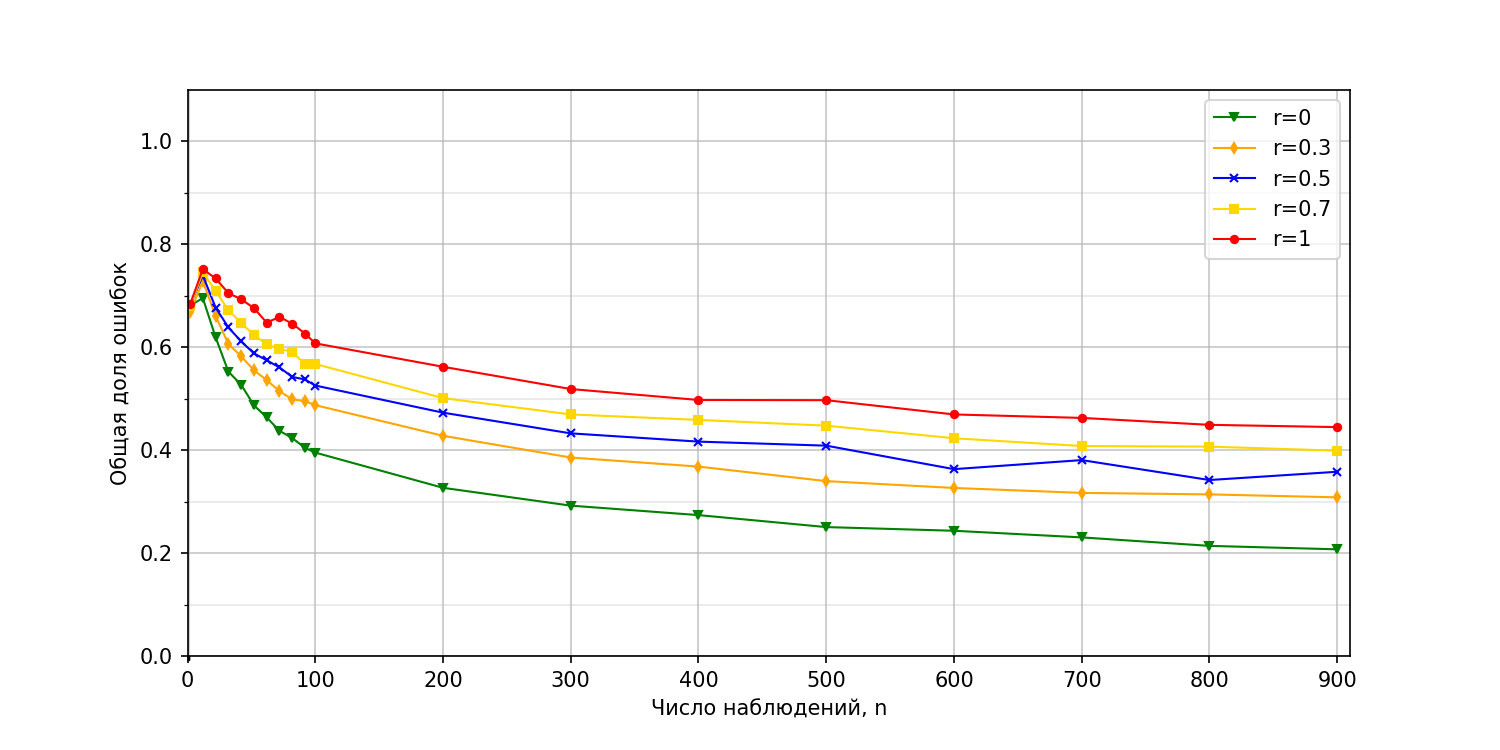
\includegraphics[width=\textwidth]{mc/total/pearson_total_1k_t=0-3}
         \caption{$\theta=0.3, N=24$}
     \end{subfigure}
     \vfill
     \begin{subfigure}[b]{0.49\textwidth}
         \centering
         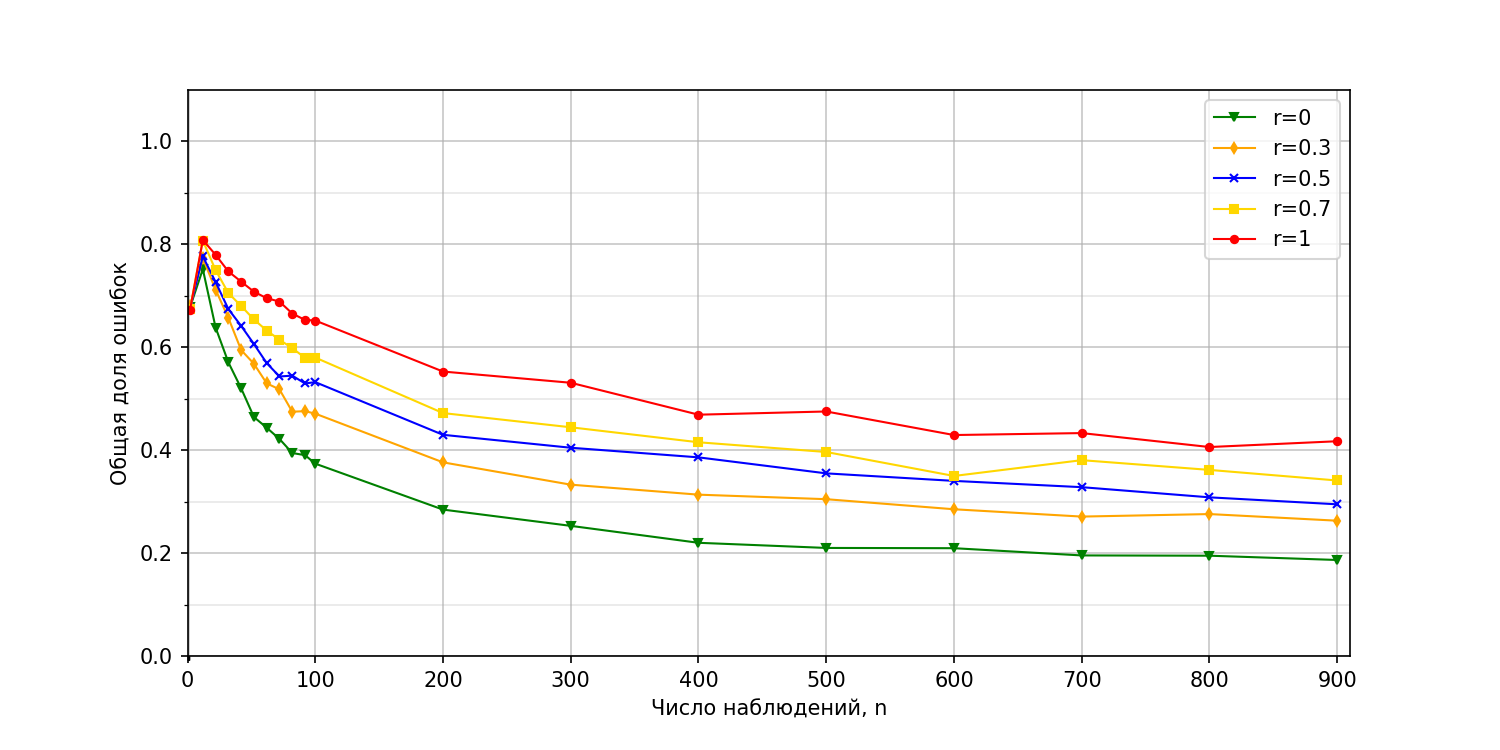
\includegraphics[width=\textwidth]{mc/total/pearson_total_1k_t=0-5}
         \caption{$\theta=0.5, N=10$}
     \end{subfigure}
     \hfill
     \begin{subfigure}[b]{0.49\textwidth}
         \centering
         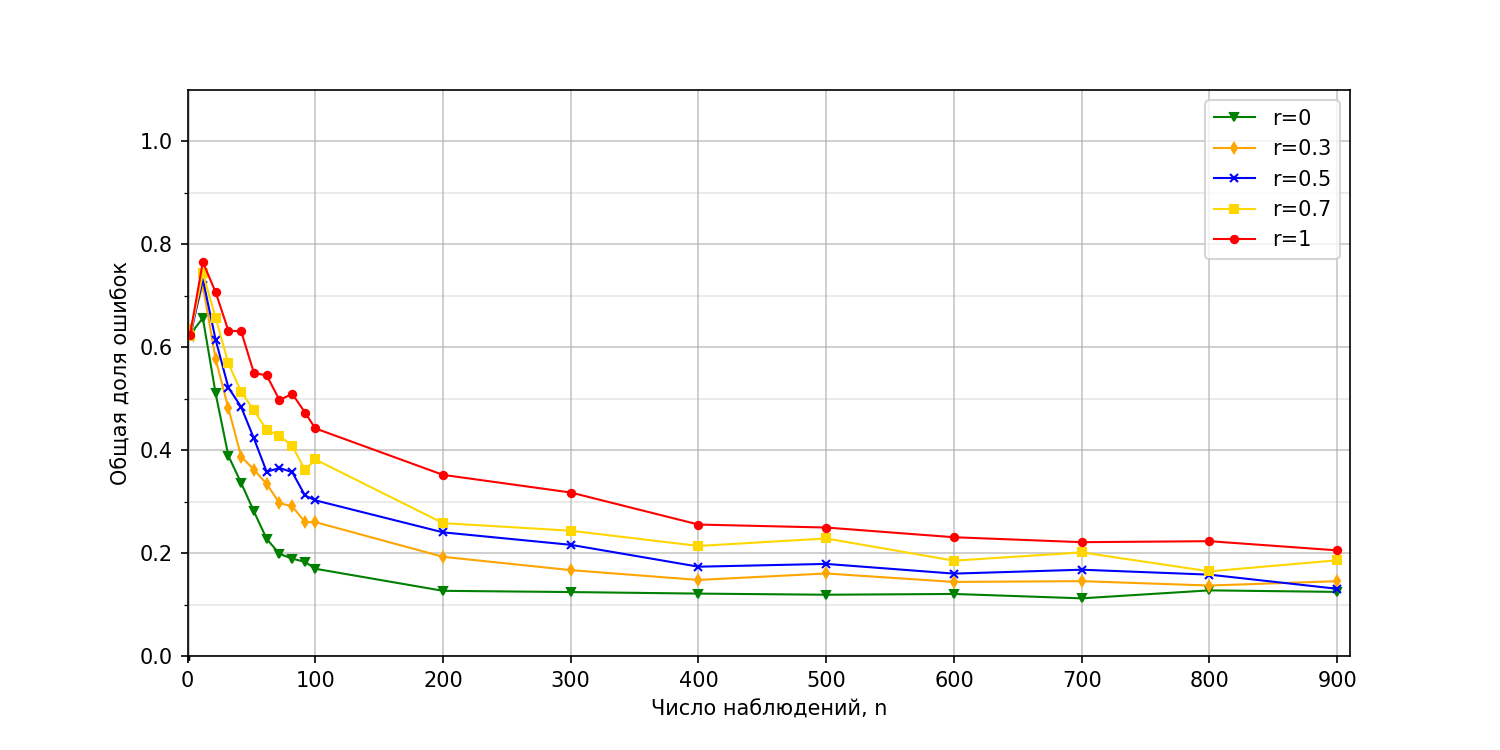
\includegraphics[width=\textwidth]{mc/total/pearson_total_1k_t=0-7}
         \caption{$\theta=0.7, N=3$}
     \end{subfigure}
    
        \caption{Зависимость общей доли ошибок от $n$,  MC}
        \label{fig:exp/mc/total_1k}
\end{figure}  

Для меры близости на основе вероятности совпадения знаков на рисунке на рисунке \ref{fig:exp/mc/signs_ratio_total} представлен график зависимости общей доли ошибки от параметра $r$ при различных $n$. Также как и для корреляции Пирсона, ошибка больше при средних значениях порога $\theta$.

\begin{figure}[H]
     \centering
     \begin{subfigure}[b]{0.49\textwidth}
         \centering
         \includegraphics[width=\textwidth]{mc/total/signs_total_ratio_t=0-1}
         \caption{$\theta=0.1, \theta_\gamma=0.53, N=55$}
     \end{subfigure}
     \hfill
     \begin{subfigure}[b]{0.49\textwidth}
         \centering
         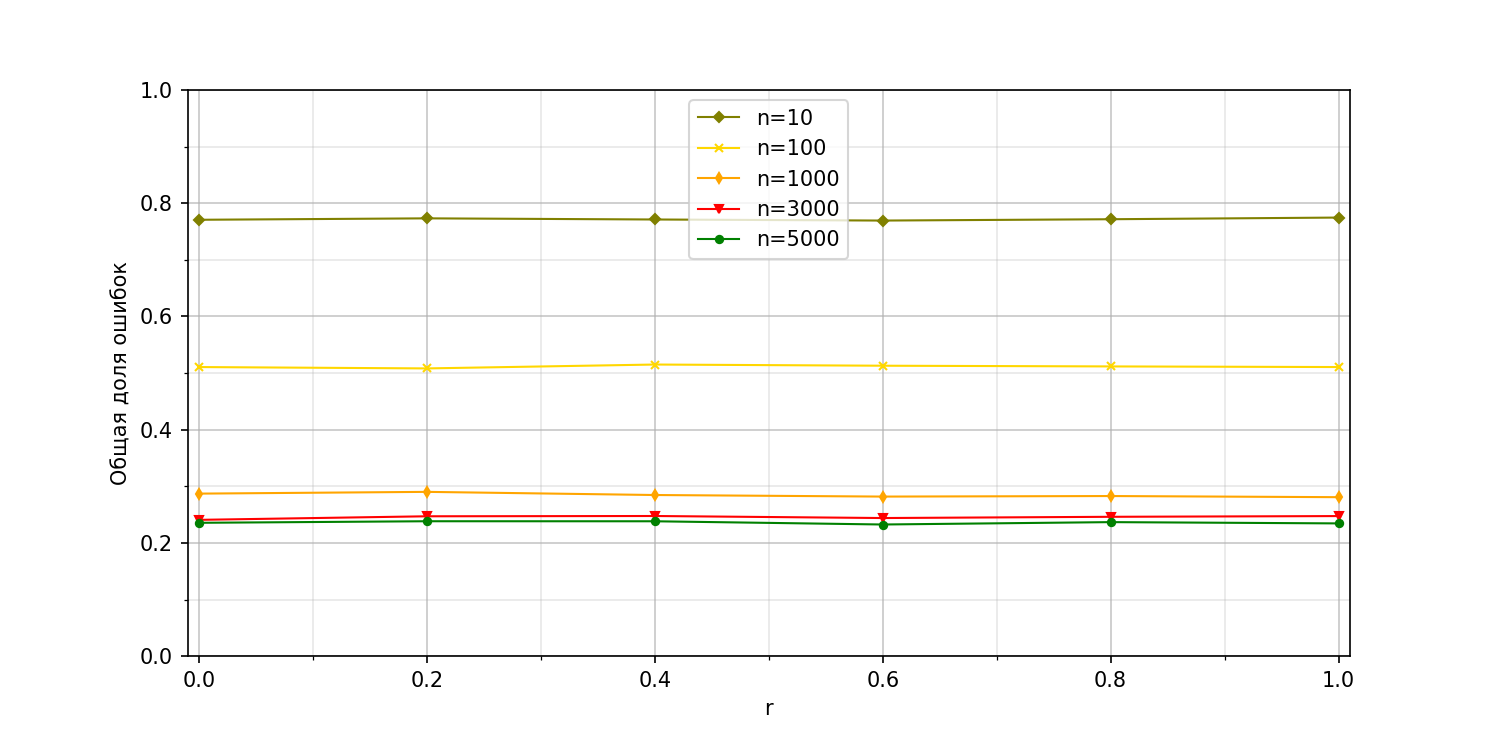
\includegraphics[width=\textwidth]{mc/total/signs_total_ratio_t=0-3}
         \caption{$\theta=0.3, \theta_\gamma=0.6, N=25$}
     \end{subfigure}
     \vfill
     \begin{subfigure}[b]{0.49\textwidth}
         \centering
         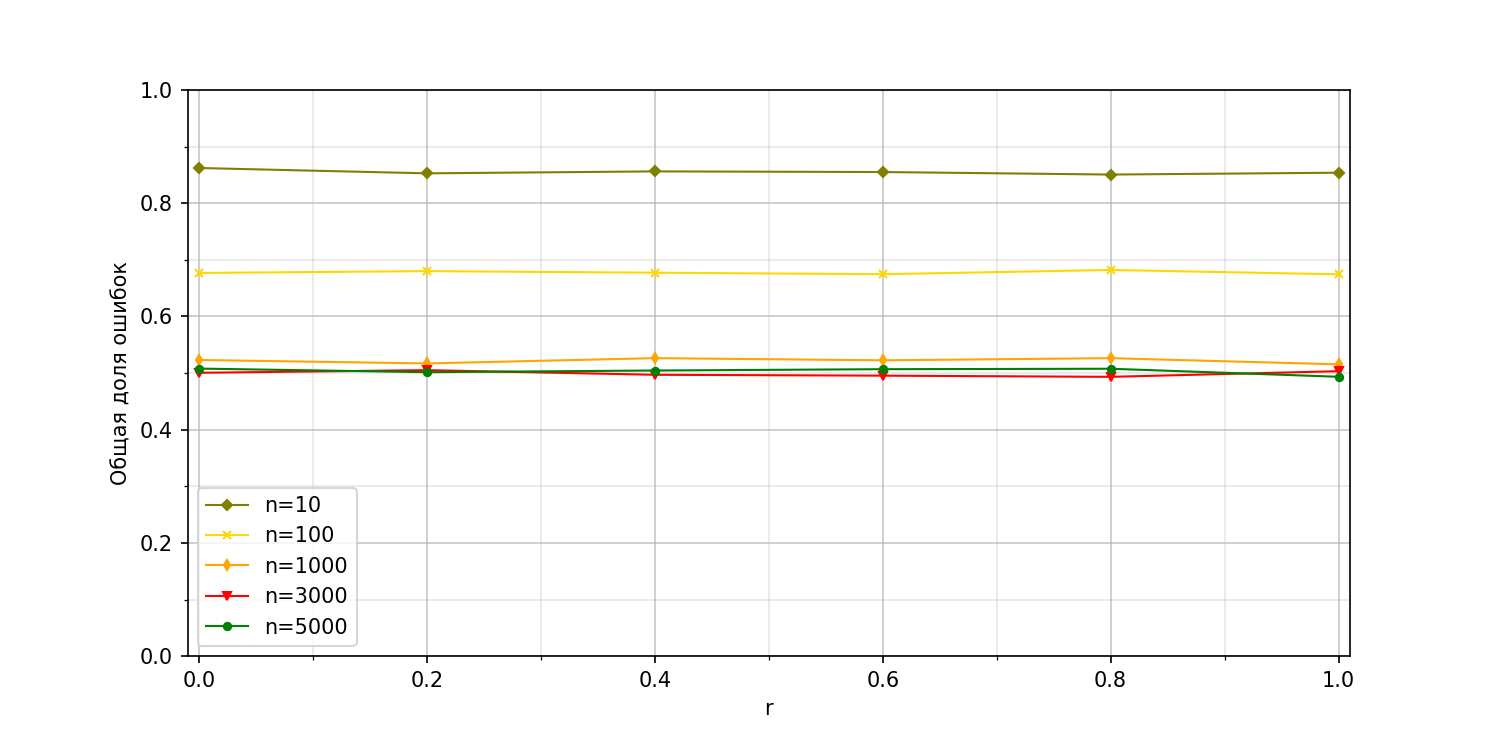
\includegraphics[width=\textwidth]{mc/total/signs_total_ratio_t=0-5}
         \caption{$\theta=0.5, \theta_\gamma=0.67, N=10$}
     \end{subfigure}
     \hfill
     \begin{subfigure}[b]{0.49\textwidth}
         \centering
         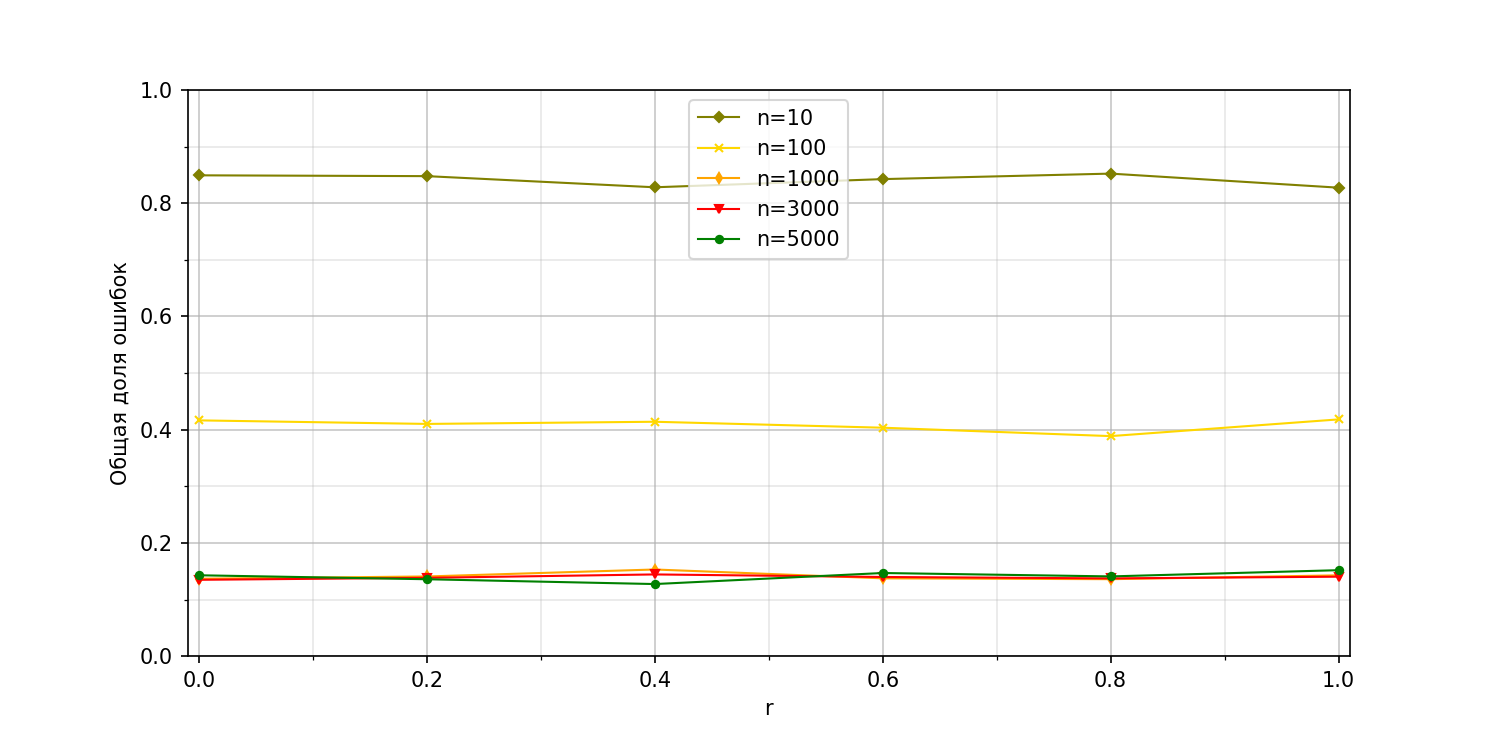
\includegraphics[width=\textwidth]{mc/total/signs_total_ratio_t=0-7}
         \caption{$\theta=0.7,\theta_\gamma=0.75, N=4$}
     \end{subfigure}

        \caption{Зависимость общей доли ошибок от $r$ для знаков, MC}
        \label{fig:exp/mc/signs_ratio_total}
\end{figure}  

На графике \ref{fig:exp/mc/pearson_signs} сравниваются значения ошибок при использовании корреляции Пирсона и корреляции вероятности совпадения знаков. Заметим, что для значений $100<n<1000$ ошибка для корреляции Пирсона и $r=1$ равна примерно равна или даже превосходит ошибку при использовании вероятностей совпадения знаков. 


\begin{figure}[H]
     \centering
     \begin{subfigure}[b]{0.49\textwidth}
         \centering
         \includegraphics[width=\textwidth]{mc/total/person_signs_t=0-1}
         \caption{$\theta=0.1, \theta_\gamma=0.53$}
     \end{subfigure}
     \hfill
     \begin{subfigure}[b]{0.49\textwidth}
         \centering
         \includegraphics[width=\textwidth]{mc/total/person_signs_t=0-3}
         \caption{$\theta=0.3, \theta_\gamma=0.6$}
     \end{subfigure}
     \vfill
     \begin{subfigure}[b]{0.49\textwidth}
         \centering
         \includegraphics[width=\textwidth]{mc/total/person_signs_t=0-5}
         \caption{$\theta=0.5, \theta_\gamma=0.67$}
     \end{subfigure}
     \hfill
     \begin{subfigure}[b]{0.49\textwidth}
         \centering
         \includegraphics[width=\textwidth]{mc/total/person_signs_t=0-7}
         \caption{$\theta=0.7,\theta_\gamma=0.75$}
     \end{subfigure}

        \caption{Сравнение ошибки для обеих мер, MC}
        \label{fig:exp/mc/pearson_signs}
\end{figure}  


\subsubsection{Максимальное независимое множество}

По аналогии с максимальной кликой, мы будем рассматривать значения общей доли ошибок для разных порогов. Пороги для максимальное независимое множества будут иными: $\theta \in [0, 0.05, 0.1, 0.15]$. 

На рисунке \ref{fig:exp/mis/total_1k} изображены графики зависимость общей доли ошибки от количества наблюдений $n$ для различных значений порога. Небольшое увеличение порога приводит к существенному уменьшению ошибки.  С ростом числа наблюдений ошибка уменьшается существенно медленне, чем у рассмотренной выше максимальной клики, и не достагает порога $\mathcal{E}_0=0.1$

\begin{figure}[H]
     \centering
     \begin{subfigure}[b]{0.49\textwidth}
         \centering
         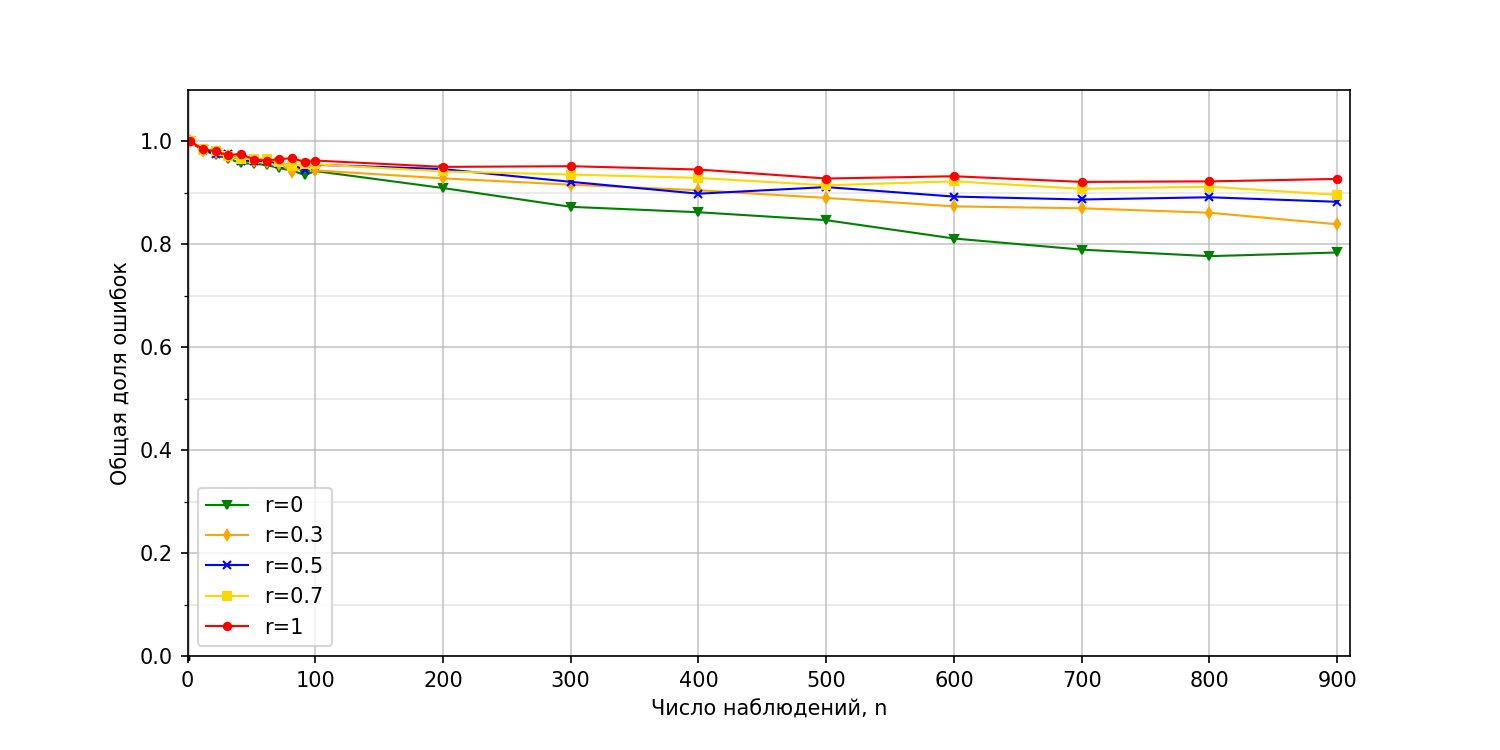
\includegraphics[width=\textwidth]{mis/total/pearson_total_1k_t=0}
         \caption{$\theta=0, N=5$}
     \end{subfigure}
     \hfill
     \begin{subfigure}[b]{0.49\textwidth}
         \centering
         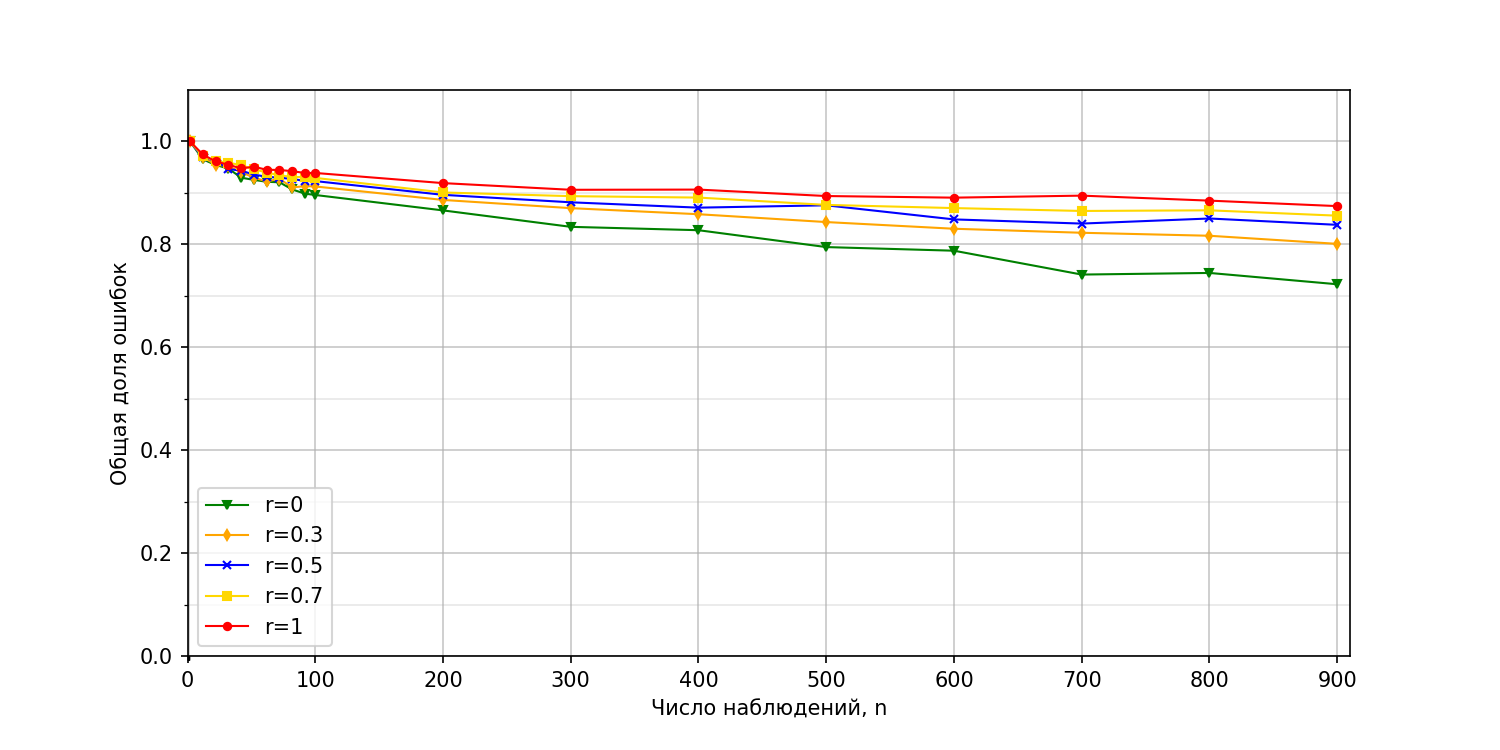
\includegraphics[width=\textwidth]{mis/total/pearson_total_1k_t=0-05}
         \caption{$\theta=0.05, N=8$}
     \end{subfigure}
     \vfill
     \begin{subfigure}[b]{0.49\textwidth}
         \centering
         \includegraphics[width=\textwidth]{mis/total/pearson_total_1k_t=0-1}
         \caption{$\theta=0.1, N=14$}
     \end{subfigure}
     \hfill
     \begin{subfigure}[b]{0.49\textwidth}
         \centering
         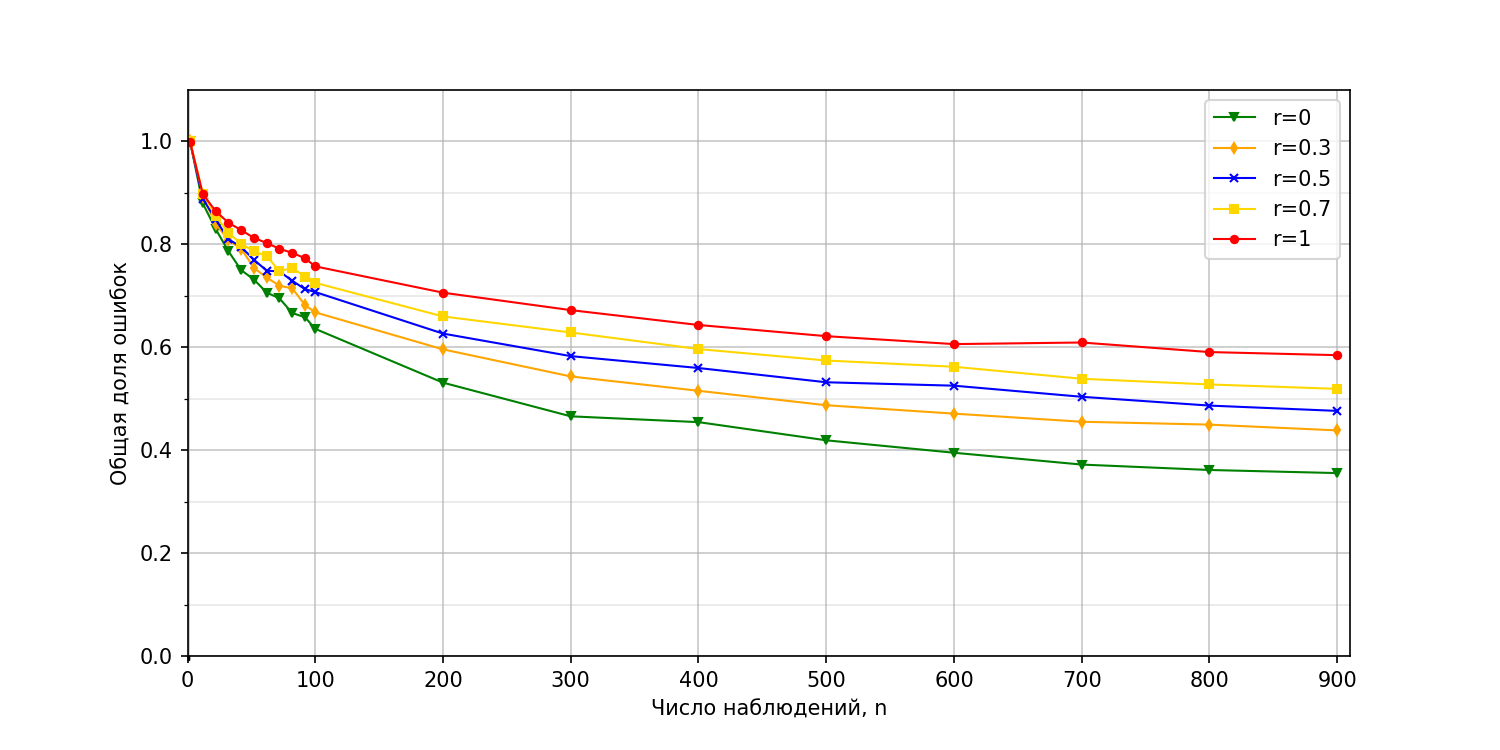
\includegraphics[width=\textwidth]{mis/total/pearson_total_1k_t=0-15}
         \caption{$\theta=0.15, N=21$}
     \end{subfigure}
    
        \caption{Зависимость общей доли ошибок от $n$,  MIS}
        \label{fig:exp/mis/total_1k}
\end{figure}  


На следующем графике \ref{fig:exp/mis/signs_ratio} представлена зависимость общей доли ошибок от параметра $r$ с вероятностю совпадения знаков в качестве меры близости. Наблюдается схожая с корреляцией Пирсона тенденция с существенном уменьшение ошибки при небольшом увеличении $\theta$. 

\begin{figure}[H]
     \centering
     \begin{subfigure}[b]{0.49\textwidth}
         \centering
         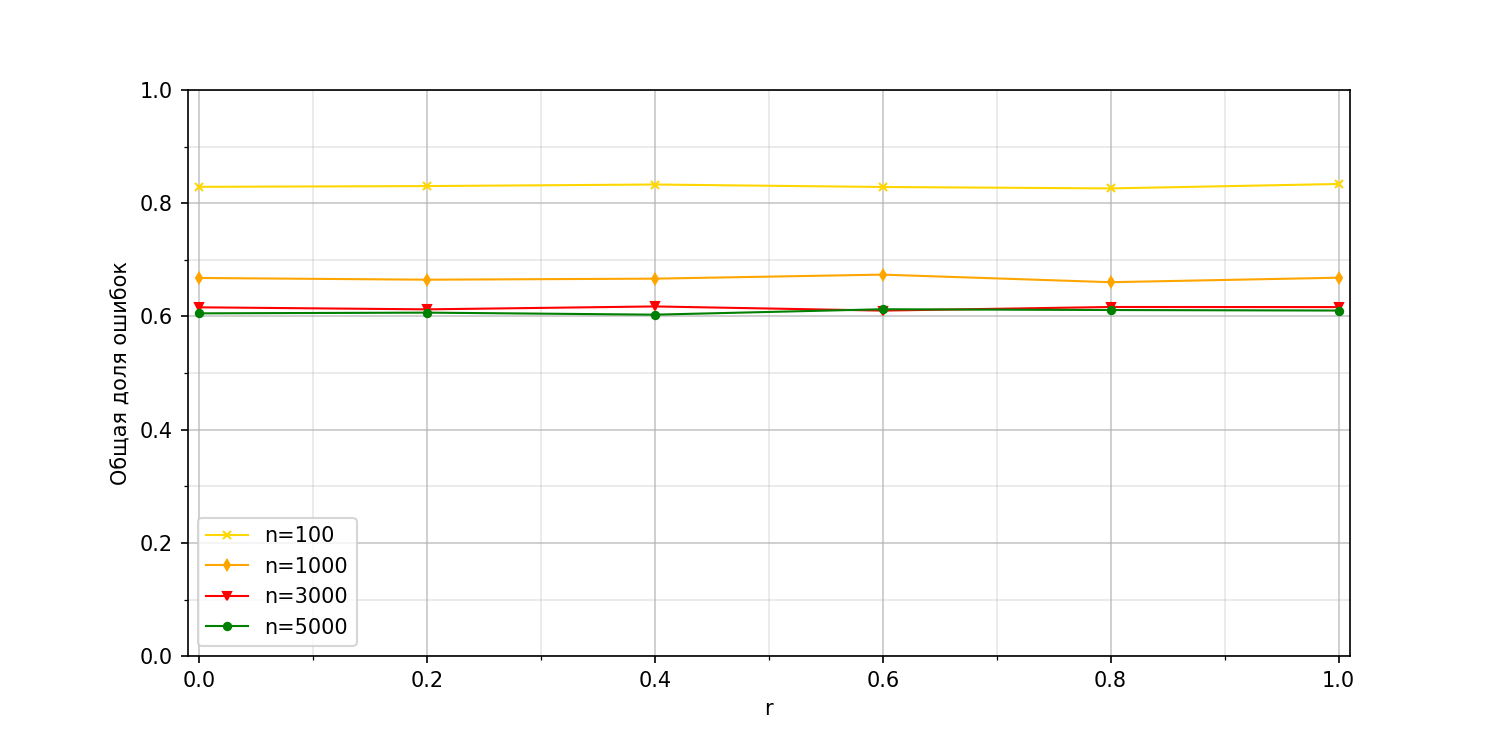
\includegraphics[width=\textwidth]{mis/total/signs_total_ratio_t=0-05}
         \caption{$\theta=0.05, \theta_\gamma=0.51, N=17$}
     \end{subfigure}
     \hfill
     \begin{subfigure}[b]{0.49\textwidth}
         \centering
         \includegraphics[width=\textwidth]{mis/total/signs_total_ratio_t=0-1}
         \caption{$\theta=0.1, \theta_\gamma=0.53, N=18$}
     \end{subfigure}
     \vfill
     \begin{subfigure}[b]{0.49\textwidth}
         \centering
         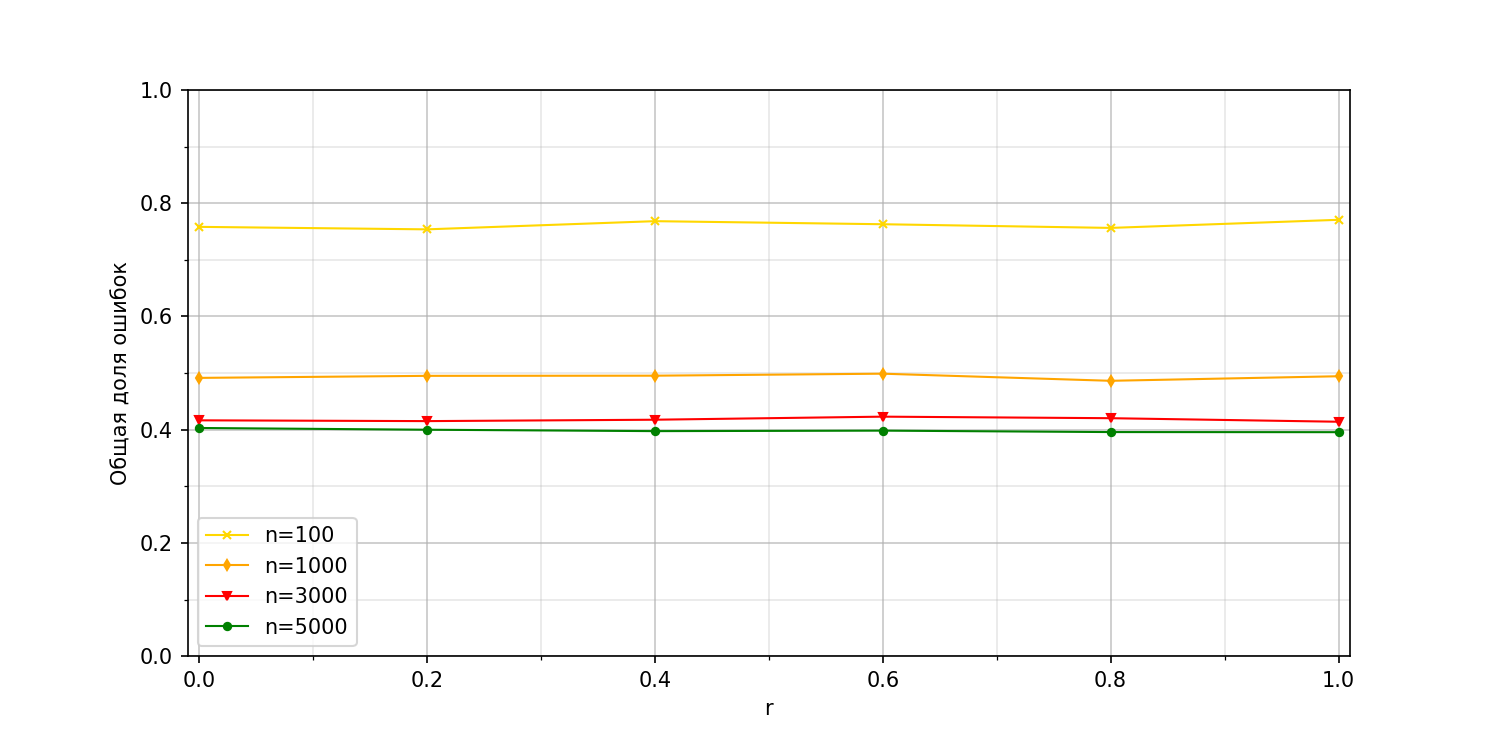
\includegraphics[width=\textwidth]{mis/total/signs_total_ratio_t=0-15}
         \caption{$\theta=0.15, \theta_\gamma=0.55, N=23$}
     \end{subfigure}
     \hfill
     \begin{subfigure}[b]{0.49\textwidth}
         \centering
         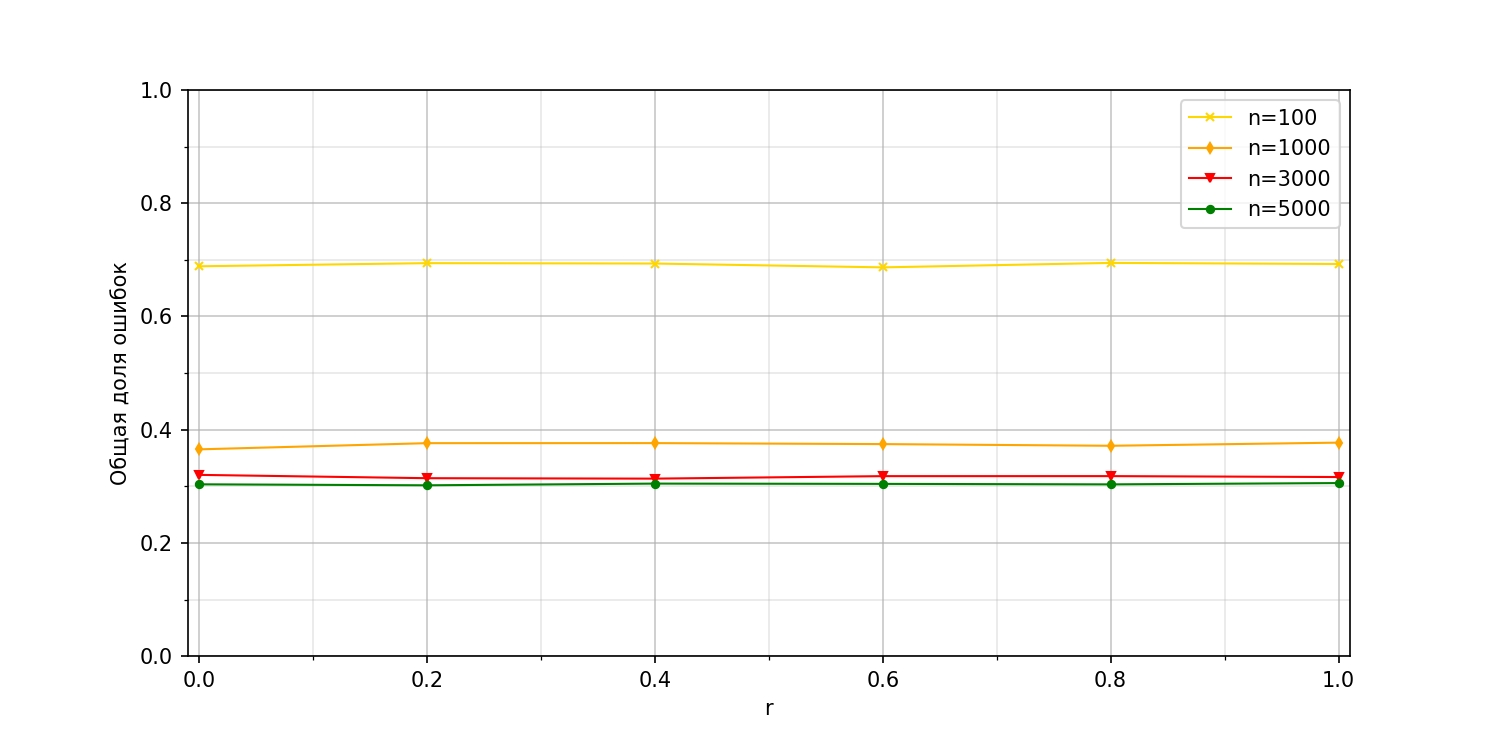
\includegraphics[width=\textwidth]{mis/total/signs_total_ratio_t=0-2}
         \caption{$\theta=0.2, \theta_\gamma=0.56, N=29$}
     \end{subfigure}
    
        \caption{Зависимость общей доли ошибок от $n$,  MIS}
        \label{fig:exp/mis/signs_ratio}
\end{figure}  

Сравнение ошибок для обеих мер представлено на график \ref{fig:exp/mis/pearson_signs}. Видно, мера вероятности совпадения знаков проявляет себя немного лучше, чем мера корреляции Пирсона.

\begin{figure}[H]
     \centering
     \begin{subfigure}[b]{0.49\textwidth}
         \centering
         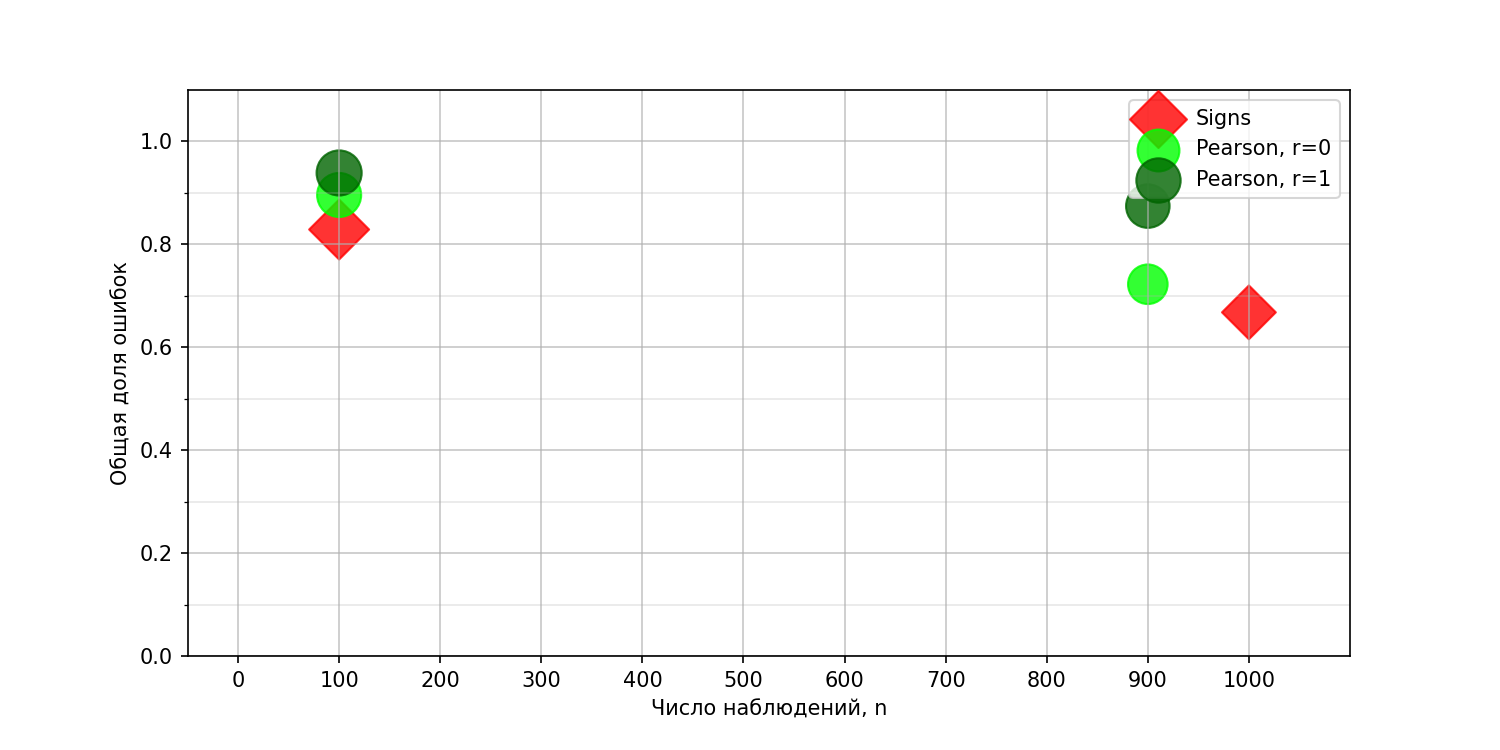
\includegraphics[width=\textwidth]{mis/total/person_signs_t=0-05}
         \caption{$\theta=0.05, \theta_\gamma=0.51$}
     \end{subfigure}
     \hfill
     \begin{subfigure}[b]{0.49\textwidth}
         \centering
         \includegraphics[width=\textwidth]{mis/total/person_signs_t=0-1}
         \caption{$\theta=0.1, \theta_\gamma=0.53$}
     \end{subfigure}
     \vfill
     \begin{subfigure}[b]{0.49\textwidth}
         \centering
         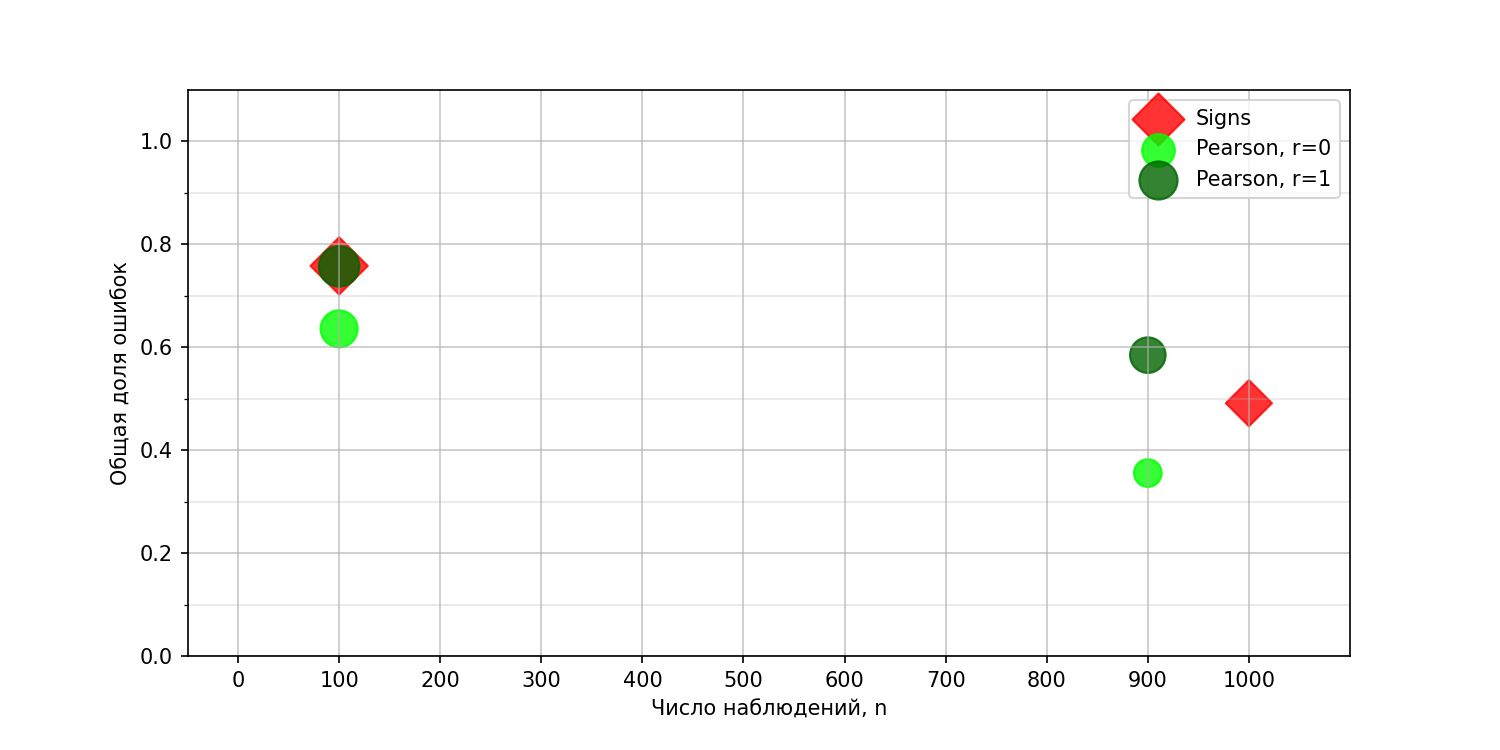
\includegraphics[width=\textwidth]{mis/total/person_signs_t=0-15}
         \caption{$\theta=0.15, \theta_\gamma=0.55$}
     \end{subfigure}

    
        \caption{Сравнение ошибки для обеих мер,  MIS}
        \label{fig:exp/mis/pearson_signs}
\end{figure}  



